%	Since the representation $J(\nu)$ of $G'=O(p,q+1)$ is multiplicity-free as a $K'$-module, we can describe its $(\mathfrak{g}',K')$-submodules by means of subsets of $\N_{+}^2$
%	for $p>1$, which parametrize the $K'$-structure of $J(\nu)$ by the spherical harmonics $\mathcal{H}^a(\Sp^{p-1})\boxtimes\mathcal{H}^b(\Sp^q)$.
%	As in \cite{howe1993homogeneous}, we also indicate the Jordan--H\"older series (socle filtrations) of $J(\nu)$ by using arrows.
%	We then have:
%\begin{theorem}[images of SBOs]
%	The regular SBO $R_{\lambda,\nu}^X:I(\lambda)\to J(\nu)$ is surjective,
%	unless $\nu\in\Z$. In the latter case, the images of the underlying $(\mathfrak{g},K)$-module $I(\lambda)_K$ under
%	$R_{\lambda,\nu}^X$ are given as follows (here we set $l:=\frac{1}{2}\left( \nu-\lambda \right)\in\N$ for $(\lambda,\nu)\in//$ and $k:=\frac{1}{2}\left( n-1-\lambda-\nu \right)
%	\in\N$ for
%	$(\lambda,\nu)\in\backslash\backslash$; the barriers $A^{\pm\pm}$ are defined as in \cite{howe1993homogeneous}): \\
%	for $p>1$:
%\end{theorem}
%\begin{enumerate}[(1)]
%	\item Suppose $p\in2\N_++1$ and $q\in2\Z$. Then, if $\nu\in2\Z,0<\nu<n-1$, $R_{\lambda,\nu}^X$ is surjective. Otherwise,\newpage
%		\hspace*{-1cm}\begin{figure}[h]
%			\noindent\begin{tabular}{m{1.6cm}rrr}
%	      $(\lambda,\nu)\in$&$\mybra{//\cup\backslash\backslash}^c$ & $\backslash\backslash-//$  & $//\cap\backslash\backslash,k> l$\\[0pt]
%	      {\vspace{-3cm} $ \begin{array}{l}
%	      \nu\teven\\ \nu\le0
%      \end{array}$}&{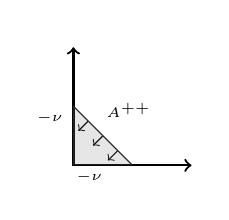
\begin{tikzpicture}[scale=0.5]
\draw [<->,thick] (0.0,3.0) node (yaxis) [above] {}
	|- (3.0,0.0) node (xaxis) [below] {};
\draw (0,1.5)  -- (1.5,0) ;
\draw [->] (0.375,1.125) -- (0.125,0.875);
\draw [->] (0.75,0.75) -- (0.5,0.5);
\draw [->] (1.125,0.375) -- (0.875,0.125);
\node at (1.4,1.4) {\tiny $A^{++}$};
\node at (0.3999999999999999,-0.3) {\tiny $-\nu$};
\node at (-0.6,1.2) {\tiny $-\nu$};
\draw [fill=gray,opacity=0.2,gray] (1.5,0.0) -- (0.0,1.5) -- (0.0,0.0) ;
\end{tikzpicture}}
&\hspace{-0.5cm}{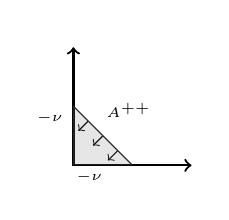
\begin{tikzpicture}[scale=0.5]
\draw [<->,thick] (0.0,3.0) node (yaxis) [above] {}
	|- (3.0,0.0) node (xaxis) [below] {};
\draw (0,1.5)  -- (1.5,0) ;
\draw [->] (0.375,1.125) -- (0.125,0.875);
\draw [->] (0.75,0.75) -- (0.5,0.5);
\draw [->] (1.125,0.375) -- (0.875,0.125);
\node at (1.4,1.4) {\tiny $A^{++}$};
\node at (0.3999999999999999,-0.3) {\tiny $-\nu$};
\node at (-0.6,1.2) {\tiny $-\nu$};
\draw [fill=gray,opacity=0.2,gray] (1.5,0.0) -- (0.0,1.5) -- (0.0,0.0) ;
\end{tikzpicture}}
&\hspace{-0.5cm}{\begin{tikzpicture}[scale=0.5]
\draw [<->,thick] (0.0,3.0) node (yaxis) [above] {}
	|- (3.0,0.0) node (xaxis) [below] {};
\draw (0,1.5)  -- (1.5,0) ;
\draw [->] (0.375,1.125) -- (0.125,0.875);
\draw [->] (0.75,0.75) -- (0.5,0.5);
\draw [->] (1.125,0.375) -- (0.875,0.125);
\node at (1.4,1.4) {\tiny $A^{++}$};
\node at (0.3999999999999999,-0.3) {\tiny $-\nu$};
\node at (-0.6,1.2) {\tiny $-\nu$};
\draw [pattern=north east lines, pattern color=green!50!black] (3.0,0.0) -- (3.0,3.0) -- (0.0,3.0) -- (0.0,0.0) ;
\draw (0,1.5)  -- (1.5,0) ;
\draw [->] (0.375,1.125) -- (0.125,0.875);
\draw [->] (0.75,0.75) -- (0.5,0.5);
\draw [->] (1.125,0.375) -- (0.875,0.125);
\node at (1.4,1.4) {\tiny $A^{++}$};
\node at (0.3999999999999999,-0.3) {\tiny $-\nu$};
\node at (-0.6,1.2) {\tiny $-\nu$};
\draw [pattern=north west lines, pattern color=purple] (1.5,0.0) -- (0.0,1.5) -- (0.0,0.0) ;
\end{tikzpicture}}
\\[0pt]
%      \vspace{-3cm}$\begin{array}{l}
%	      \nu\todd\\ \nu\le\frac{n-3}{2}
%      \end{array}$&{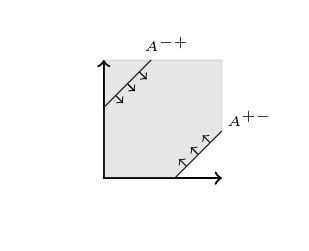
\begin{tikzpicture}[scale=0.5]
\draw [<->,thick] (0.0,3.0) node (yaxis) [above] {}
	|- (3.0,0.0) node (xaxis) [below] {};
\draw (1.8,0.0) -- (3.0,1.2) ;
\draw [->] (2.1,0.3) -- (1.9100000000000001,0.49);
\draw [->] (2.4,0.6) -- (2.21,0.79);
\draw [->] (2.7,0.8999999999999999) -- (2.5100000000000002,1.0899999999999999);
\node at (3.7,1.5) {\tiny $A^{+-}$};
\node at (1.8,-0.9) {\tiny $$};
\draw [fill=gray,opacity=0.2,gray] (1.8,0.0) -- (3.0,1.2) -- (3.0,3.0) -- (1.2,3.0) -- (0.0,1.8) -- (0.0,0.0) ;
\draw (0.0,1.8) -- (1.2,3.0) ;
\draw [->] (0.3,2.1) -- (0.49,1.9100000000000001);
\draw [->] (0.6,2.4) -- (0.79,2.21);
\draw [->] (0.8999999999999999,2.7) -- (1.0899999999999999,2.5100000000000002);
\node at (1.6,3.4) {\tiny $A^{-+}$};
\node at (-1.7,1.9000000000000001) {\tiny $$};
\draw [fill=gray,opacity=0.2,gray] (0.0,1.8) -- (1.2,3.0) -- (0.0,3.0) ;
\end{tikzpicture}}
&\hspace{-0.5cm}{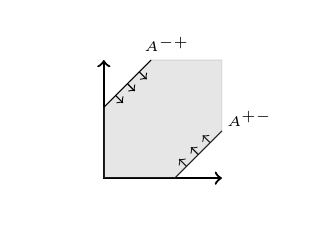
\begin{tikzpicture}[scale=0.5]
\draw [<->,thick] (0.0,3.0) node (yaxis) [above] {}
	|- (3.0,0.0) node (xaxis) [below] {};
\draw (1.8,0.0) -- (3.0,1.2) ;
\draw [->] (2.1,0.3) -- (1.9100000000000001,0.49);
\draw [->] (2.4,0.6) -- (2.21,0.79);
\draw [->] (2.7,0.8999999999999999) -- (2.5100000000000002,1.0899999999999999);
\node at (3.7,1.5) {\tiny $A^{+-}$};
\node at (1.8,-0.9) {\tiny $$};
\draw [fill=gray,opacity=0.2,gray] (1.8,0.0) -- (3.0,1.2) -- (3.0,3.0) -- (1.2,3.0) -- (0.0,1.8) -- (0.0,0.0) ;
\draw (0.0,1.8) -- (1.2,3.0) ;
\draw [->] (0.3,2.1) -- (0.49,1.9100000000000001);
\draw [->] (0.6,2.4) -- (0.79,2.21);
\draw [->] (0.8999999999999999,2.7) -- (1.0899999999999999,2.5100000000000002);
\node at (1.6,3.4) {\tiny $A^{-+}$};
\node at (-1.7,1.9000000000000001) {\tiny $$};
\end{tikzpicture}}
&\hspace{-0.5cm}{\begin{tikzpicture}[scale=0.5]
\draw [<->,thick] (0.0,3.0) node (yaxis) [above] {}
	|- (3.0,0.0) node (xaxis) [below] {};
\draw (1.8,0.0) -- (3.0,1.2) ;
\draw [->] (2.1,0.3) -- (1.9100000000000001,0.49);
\draw [->] (2.4,0.6) -- (2.21,0.79);
\draw [->] (2.7,0.8999999999999999) -- (2.5100000000000002,1.0899999999999999);
\node at (3.7,1.5) {\tiny $A^{+-}$};
\node at (1.8,-0.9) {\tiny $$};
\draw [pattern=north west lines, pattern color=purple] (1.8,0.0) -- (3.0,1.2) -- (3.0,3.0) -- (0.0,3.0) -- (0.0,0.0) ;
\draw (0.0,1.8) -- (1.2,3.0) ;
\draw [->] (0.3,2.1) -- (0.49,1.9100000000000001);
\draw [->] (0.6,2.4) -- (0.79,2.21);
\draw [->] (0.8999999999999999,2.7) -- (1.0899999999999999,2.5100000000000002);
\node at (1.6,3.4) {\tiny $A^{-+}$};
\node at (-1.7,1.9000000000000001) {\tiny $$};
\draw [pattern=north east lines, pattern color=green!50!black] (3.0,0.0) -- (3.0,3.0) -- (0.0,3.0) -- (0.0,0.0) ;
\end{tikzpicture}}
\\[0pt]
%	      $(\lambda,\nu)\in$&$\mybra{//\cup\backslash\backslash}^c$ && $//\cap\backslash\backslash,k=l$\\[0pt]
%	      \vspace{-3cm}$\begin{array}{l}\nu\todd\\\nu=\frac{n-1}{2}
%	      \end{array}$&{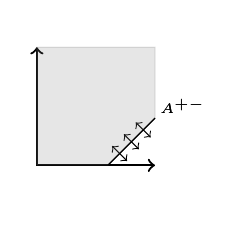
\begin{tikzpicture}[scale=0.5]
\draw [<->,thick] (0.0,3.0) node (yaxis) [above] {}
	|- (3.0,0.0) node (xaxis) [below] {};
\draw (1.8,0.0) -- (3.0,1.2) ;
\draw [->] (2.1,0.3) -- (1.9100000000000001,0.49);
\draw [->] (2.4,0.6) -- (2.21,0.79);
\draw [->] (2.7,0.8999999999999999) -- (2.5100000000000002,1.0899999999999999);
\node at (3.7,1.5) {\tiny $A^{+-}$};
\node at (1.8,-0.9) {\tiny $$};
\draw [fill=gray,opacity=0.2,gray] (1.8,0.0) -- (3.0,1.2) -- (3.0,3.0) -- (0.0,3.0) -- (0.0,0.0) ;
\draw (1.8,0.0) -- (3.0,1.2) ;
\draw [->] (2.1,0.3) -- (2.29,0.10999999999999999);
\draw [->] (2.4,0.6) -- (2.59,0.41);
\draw [->] (2.7,0.8999999999999999) -- (2.89,0.71);
\node at (3.7,1.5) {\tiny $A^{+-}$};
\node at (1.8,-0.9) {\tiny $$};
\end{tikzpicture}}
&\hspace{-0.5cm}&\hspace{-0.5cm}{\begin{tikzpicture}[scale=0.5]
\draw [<->,thick] (0.0,3.0) node (yaxis) [above] {}
	|- (3.0,0.0) node (xaxis) [below] {};
\draw (1.8,0.0) -- (3.0,1.2) ;
\draw [->] (2.1,0.3) -- (1.9100000000000001,0.49);
\draw [->] (2.4,0.6) -- (2.21,0.79);
\draw [->] (2.7,0.8999999999999999) -- (2.5100000000000002,1.0899999999999999);
\node at (3.7,1.5) {\tiny $A^{+-}$};
\node at (1.8,-0.9) {\tiny $$};
\draw [pattern=north east lines, pattern color=green!50!black] (3.0,0.0) -- (3.0,3.0) -- (0.0,3.0) -- (0.0,0.0) ;
\draw (1.8,0.0) -- (3.0,1.2) ;
\draw [->] (2.1,0.3) -- (2.29,0.10999999999999999);
\draw [->] (2.4,0.6) -- (2.59,0.41);
\draw [->] (2.7,0.8999999999999999) -- (2.89,0.71);
\node at (3.7,1.5) {\tiny $A^{+-}$};
\node at (1.8,-0.9) {\tiny $$};
\draw [pattern=north west lines, pattern color=purple] (1.8,0.0) -- (3.0,1.2) -- (3.0,3.0) -- (0.0,3.0) -- (0.0,0.0) ;
\end{tikzpicture}}
\\[0pt]
%	      $(\lambda,\nu)\in$&$\mybra{//\cup\backslash\backslash}^c$ & $//-\backslash\backslash$  & $//\cap\backslash\backslash,k< l$\\[0pt]
%	      \vspace{-3cm}$\begin{array}{l}\nu\teven\\\nu\ge{n-1}\end{array}$&{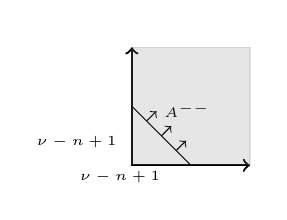
\begin{tikzpicture}[scale=0.5]
\draw [<->,thick] (0.0,3.0) node (yaxis) [above] {}
	|- (3.0,0.0) node (xaxis) [below] {};
\draw (0,1.5)  -- (1.5,0) ;
\draw [->] (0.375,1.125) -- (0.625,1.375);
\draw [->] (0.75,0.75) -- (1.0,1.0);
\draw [->] (1.125,0.375) -- (1.375,0.625);
\node at (-1.4,0.6) {\tiny $\nu-n+1$};
\node at (-0.30000000000000004,-0.3) {\tiny $\nu-n+1$};
\node at (1.4,1.4) {\tiny $A^{--}$};
\draw [fill=gray,opacity=0.2,gray] (3.0,0.0) -- (3.0,3.0) -- (0.0,3.0) -- (0.0,0.0) ;
\end{tikzpicture}}
&\hspace{-0.5cm}{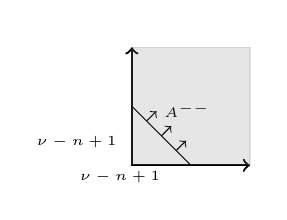
\begin{tikzpicture}[scale=0.5]
\draw [<->,thick] (0.0,3.0) node (yaxis) [above] {}
	|- (3.0,0.0) node (xaxis) [below] {};
\draw (0,1.5)  -- (1.5,0) ;
\draw [->] (0.375,1.125) -- (0.625,1.375);
\draw [->] (0.75,0.75) -- (1.0,1.0);
\draw [->] (1.125,0.375) -- (1.375,0.625);
\node at (-1.4,0.6) {\tiny $\nu-n+1$};
\node at (-0.30000000000000004,-0.3) {\tiny $\nu-n+1$};
\node at (1.4,1.4) {\tiny $A^{--}$};
\draw [fill=gray,opacity=0.2,gray] (3.0,0.0) -- (3.0,3.0) -- (0.0,3.0) -- (0.0,0.0) ;
\end{tikzpicture}}
&\hspace{-0.5cm}{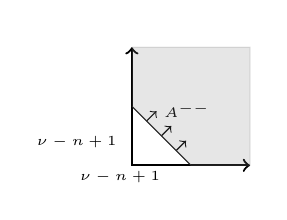
\begin{tikzpicture}[scale=0.5]
\draw [<->,thick] (0.0,3.0) node (yaxis) [above] {}
	|- (3.0,0.0) node (xaxis) [below] {};
\draw (0,1.5)  -- (1.5,0) ;
\draw [->] (0.375,1.125) -- (0.625,1.375);
\draw [->] (0.75,0.75) -- (1.0,1.0);
\draw [->] (1.125,0.375) -- (1.375,0.625);
\node at (-1.4,0.6) {\tiny $\nu-n+1$};
\node at (-0.30000000000000004,-0.3) {\tiny $\nu-n+1$};
\node at (1.4,1.4) {\tiny $A^{--}$};
\draw [fill=gray,opacity=0.2,gray] (0.0,1.5) -- (1.5,0.0) -- (3.0,0.0) -- (3.0,3.0) -- (0.0,3.0) ;
\end{tikzpicture}}
\\[0pt]
%	    \end{tabular}
%	  \end{figure}
%		\begin{figure}[h]
%			\noindent\begin{tabular}{m{1.3cm}rrr}
%	      $(\lambda,\nu)\in$&$\mybra{//\cup\backslash\backslash}^c$ & $//-\backslash\backslash$  & $//\cap\backslash\backslash,k< l$\\[0pt]
%	      \vspace{-3cm}$\begin{array}{l}\nu\todd\\\nu\ge\frac{n+1}{2}\end{array}$&{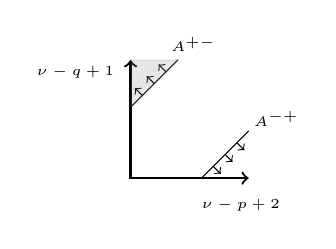
\begin{tikzpicture}[scale=0.5]
\draw [<->,thick] (0.0,3.0) node (yaxis) [above] {}
	|- (3.0,0.0) node (xaxis) [below] {};
\draw (1.8,0.0) -- (3.0,1.2) ;
\draw [->] (2.1,0.3) -- (2.29,0.10999999999999999);
\draw [->] (2.4,0.6) -- (2.59,0.41);
\draw [->] (2.7,0.8999999999999999) -- (2.89,0.71);
\node at (3.7,1.5) {\tiny $A^{-+}$};
\node at (2.8,-0.7) {\tiny $\nu-p+2$};
\draw (0.0,1.8) -- (1.2,3.0) ;
\draw [->] (0.3,2.1) -- (0.10999999999999999,2.29);
\draw [->] (0.6,2.4) -- (0.41,2.59);
\draw [->] (0.8999999999999999,2.7) -- (0.71,2.89);
\node at (1.6,3.4) {\tiny $A^{+-}$};
\node at (-1.4,2.7) {\tiny $\nu-q+1$};
\draw [fill=gray,opacity=0.2,gray] (0.0,1.8) -- (1.2,3.0) -- (0.0,3.0) ;
\end{tikzpicture}}
&\hspace{-0.5cm}{\begin{tikzpicture}[scale=0.5]
\draw [<->,thick] (0.0,3.0) node (yaxis) [above] {}
	|- (3.0,0.0) node (xaxis) [below] {};
\draw (1.8,0.0) -- (3.0,1.2) ;
\draw [->] (2.1,0.3) -- (2.29,0.10999999999999999);
\draw [->] (2.4,0.6) -- (2.59,0.41);
\draw [->] (2.7,0.8999999999999999) -- (2.89,0.71);
\node at (3.7,1.5) {\tiny $A^{-+}$};
\node at (2.8,-0.7) {\tiny $\nu-p+2$};
\draw [pattern=north east lines, pattern color=green!50!black] (3.0,0.0) -- (3.0,3.0) -- (0.0,3.0) -- (0.0,0.0) ;
\draw (0.0,1.8) -- (1.2,3.0) ;
\draw [->] (0.3,2.1) -- (0.10999999999999999,2.29);
\draw [->] (0.6,2.4) -- (0.41,2.59);
\draw [->] (0.8999999999999999,2.7) -- (0.71,2.89);
\node at (1.6,3.4) {\tiny $A^{+-}$};
\node at (-1.4,2.7) {\tiny $\nu-q+1$};
\draw [pattern=north west lines, pattern color=purple] (0.0,1.8) -- (1.2,3.0) -- (0.0,3.0) ;
\end{tikzpicture}}
&\hspace{-0.5cm}{\begin{tikzpicture}[scale=0.5]
\draw [<->,thick] (0.0,3.0) node (yaxis) [above] {}
	|- (3.0,0.0) node (xaxis) [below] {};
\draw (1.8,0.0) -- (3.0,1.2) ;
\draw [->] (2.1,0.3) -- (2.29,0.10999999999999999);
\draw [->] (2.4,0.6) -- (2.59,0.41);
\draw [->] (2.7,0.8999999999999999) -- (2.89,0.71);
\node at (3.7,1.5) {\tiny $A^{-+}$};
\node at (2.8,-0.7) {\tiny $\nu-p+2$};
\draw [pattern=north east lines, pattern color=green!50!black] (1.8,0.0) -- (3.0,1.2) -- (3.0,0.0) ;
\draw (0.0,1.8) -- (1.2,3.0) ;
\draw [->] (0.3,2.1) -- (0.10999999999999999,2.29);
\draw [->] (0.6,2.4) -- (0.41,2.59);
\draw [->] (0.8999999999999999,2.7) -- (0.71,2.89);
\node at (1.6,3.4) {\tiny $A^{+-}$};
\node at (-1.4,2.7) {\tiny $\nu-q+1$};
\draw [pattern=north east lines, pattern color=green!50!black] (0.0,1.8) -- (1.2,3.0) -- (0.0,3.0) ;
\draw (0.0,1.8) -- (1.2,3.0) ;
\draw [->] (0.3,2.1) -- (0.10999999999999999,2.29);
\draw [->] (0.6,2.4) -- (0.41,2.59);
\draw [->] (0.8999999999999999,2.7) -- (0.71,2.89);
\node at (1.6,3.4) {\tiny $A^{+-}$};
\node at (-1.4,2.7) {\tiny $\nu-q+1$};
\draw [pattern=north west lines, pattern color=purple] (0.0,1.8) -- (1.2,3.0) -- (0.0,3.0) ;
\end{tikzpicture}}
\\[25pt]
%	    \end{tabular}
%	  \end{figure}
%	\item Suppose $p,q\in\odd$ and $p>1$. Then,\clearpage
%		\begin{figure}[h]
%			\noindent\begin{tabular}{m{1.3cm}rrr}
%			$(\lambda,\nu)\in$&$\mybra{\ss\cup\bb}^c$ & $\bb-\ss$  & $\ss-\bb$\\[0pt]
%			\tevenText{\le0}&{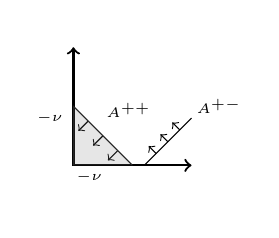
\begin{tikzpicture}[scale=0.5]
\draw [<->,thick] (0.0,3.0) node (yaxis) [above] {}
	|- (3.0,0.0) node (xaxis) [below] {};
\draw (0,1.5)  -- (1.5,0) ;
\draw [->] (0.375,1.125) -- (0.125,0.875);
\draw [->] (0.75,0.75) -- (0.5,0.5);
\draw [->] (1.125,0.375) -- (0.875,0.125);
\node at (1.4,1.4) {\tiny $A^{++}$};
\node at (0.3999999999999999,-0.3) {\tiny $-\nu$};
\node at (-0.6,1.2) {\tiny $-\nu$};
\draw [fill=gray,opacity=0.2,gray] (1.5,0.0) -- (0.0,1.5) -- (0.0,0.0) ;
\draw (1.8,0.0) -- (3.0,1.2) ;
\draw [->] (2.1,0.3) -- (1.9100000000000001,0.49);
\draw [->] (2.4,0.6) -- (2.21,0.79);
\draw [->] (2.7,0.8999999999999999) -- (2.5100000000000002,1.0899999999999999);
\node at (3.7,1.5) {\tiny $A^{+-}$};
\node at (1.8,-0.9) {\tiny $$};
\end{tikzpicture}}
&\hspace{-0.5cm}{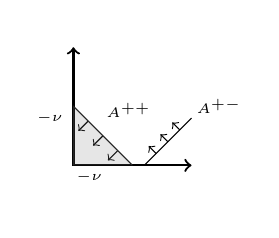
\begin{tikzpicture}[scale=0.5]
\draw [<->,thick] (0.0,3.0) node (yaxis) [above] {}
	|- (3.0,0.0) node (xaxis) [below] {};
\draw (0,1.5)  -- (1.5,0) ;
\draw [->] (0.375,1.125) -- (0.125,0.875);
\draw [->] (0.75,0.75) -- (0.5,0.5);
\draw [->] (1.125,0.375) -- (0.875,0.125);
\node at (1.4,1.4) {\tiny $A^{++}$};
\node at (0.3999999999999999,-0.3) {\tiny $-\nu$};
\node at (-0.6,1.2) {\tiny $-\nu$};
\draw [fill=gray,opacity=0.2,gray] (1.5,0.0) -- (0.0,1.5) -- (0.0,0.0) ;
\draw (1.8,0.0) -- (3.0,1.2) ;
\draw [->] (2.1,0.3) -- (1.9100000000000001,0.49);
\draw [->] (2.4,0.6) -- (2.21,0.79);
\draw [->] (2.7,0.8999999999999999) -- (2.5100000000000002,1.0899999999999999);
\node at (3.7,1.5) {\tiny $A^{+-}$};
\node at (1.8,-0.9) {\tiny $$};
\end{tikzpicture}}
&\hspace{-0.5cm}{\begin{tikzpicture}[scale=0.5]
\draw [<->,thick] (0.0,3.0) node (yaxis) [above] {}
	|- (3.0,0.0) node (xaxis) [below] {};
\draw (0,1.5)  -- (1.5,0) ;
\draw [->] (0.375,1.125) -- (0.125,0.875);
\draw [->] (0.75,0.75) -- (0.5,0.5);
\draw [->] (1.125,0.375) -- (0.875,0.125);
\node at (1.4,1.4) {\tiny $A^{++}$};
\node at (0.3999999999999999,-0.3) {\tiny $-\nu$};
\node at (-0.6,1.2) {\tiny $-\nu$};
\draw [pattern=north west lines, pattern color=purple] (1.5,0.0) -- (0.0,1.5) -- (0.0,0.0) ;
\draw (1.8,0.0) -- (3.0,1.2) ;
\draw [->] (2.1,0.3) -- (1.9100000000000001,0.49);
\draw [->] (2.4,0.6) -- (2.21,0.79);
\draw [->] (2.7,0.8999999999999999) -- (2.5100000000000002,1.0899999999999999);
\node at (3.7,1.5) {\tiny $A^{+-}$};
\node at (1.8,-0.9) {\tiny $$};
\draw [pattern=north east lines, pattern color=green!50!black] (3.0,0.0) -- (3.0,3.0) -- (0.0,3.0) -- (0.0,0.0) ;
\end{tikzpicture}}
\\[0pt]
%			\toddText{\le n-3}&{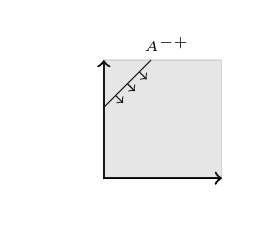
\begin{tikzpicture}[scale=0.5]
\draw [<->,thick] (0.0,3.0) node (yaxis) [above] {}
	|- (3.0,0.0) node (xaxis) [below] {};
\draw (0.0,1.8) -- (1.2,3.0) ;
\draw [->] (0.3,2.1) -- (0.49,1.9100000000000001);
\draw [->] (0.6,2.4) -- (0.79,2.21);
\draw [->] (0.8999999999999999,2.7) -- (1.0899999999999999,2.5100000000000002);
\node at (1.6,3.4) {\tiny $A^{-+}$};
\node at (-1.7,1.9000000000000001) {\tiny $$};
\draw [fill=gray,opacity=0.2,gray] (3.0,0.0) -- (3.0,3.0) -- (0.0,3.0) -- (0.0,0.0) ;
\end{tikzpicture}}
&\hspace{-0.5cm}{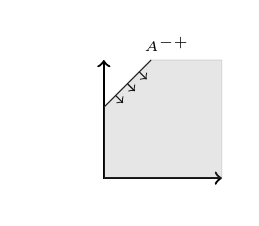
\begin{tikzpicture}[scale=0.5]
\draw [<->,thick] (0.0,3.0) node (yaxis) [above] {}
	|- (3.0,0.0) node (xaxis) [below] {};
\draw (0.0,1.8) -- (1.2,3.0) ;
\draw [->] (0.3,2.1) -- (0.49,1.9100000000000001);
\draw [->] (0.6,2.4) -- (0.79,2.21);
\draw [->] (0.8999999999999999,2.7) -- (1.0899999999999999,2.5100000000000002);
\node at (1.6,3.4) {\tiny $A^{-+}$};
\node at (-1.7,1.9000000000000001) {\tiny $$};
\draw [fill=gray,opacity=0.2,gray] (0.0,1.8) -- (1.2,3.0) -- (3.0,3.0) -- (3.0,0.0) -- (0.0,0.0) ;
\end{tikzpicture}}
&\hspace{-0.5cm}{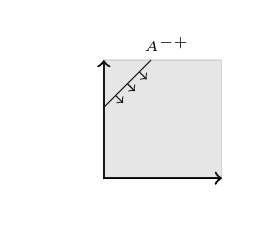
\begin{tikzpicture}[scale=0.5]
\draw [<->,thick] (0.0,3.0) node (yaxis) [above] {}
	|- (3.0,0.0) node (xaxis) [below] {};
\draw (0.0,1.8) -- (1.2,3.0) ;
\draw [->] (0.3,2.1) -- (0.49,1.9100000000000001);
\draw [->] (0.6,2.4) -- (0.79,2.21);
\draw [->] (0.8999999999999999,2.7) -- (1.0899999999999999,2.5100000000000002);
\node at (1.6,3.4) {\tiny $A^{-+}$};
\node at (-1.7,1.9000000000000001) {\tiny $$};
\draw [fill=gray,opacity=0.2,gray] (3.0,0.0) -- (3.0,3.0) -- (0.0,3.0) -- (0.0,0.0) ;
\end{tikzpicture}}
\\[0pt]
%			\tevenText{>0}&{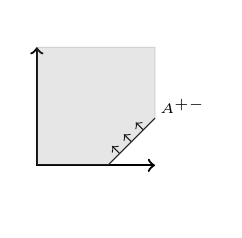
\begin{tikzpicture}[scale=0.5]
\draw [<->,thick] (0.0,3.0) node (yaxis) [above] {}
	|- (3.0,0.0) node (xaxis) [below] {};
\draw (1.8,0.0) -- (3.0,1.2) ;
\draw [->] (2.1,0.3) -- (1.9100000000000001,0.49);
\draw [->] (2.4,0.6) -- (2.21,0.79);
\draw [->] (2.7,0.8999999999999999) -- (2.5100000000000002,1.0899999999999999);
\node at (3.7,1.5) {\tiny $A^{+-}$};
\node at (1.8,-0.9) {\tiny $$};
\draw [fill=gray,opacity=0.2,gray] (1.8,0.0) -- (3.0,1.2) -- (3.0,3.0) -- (0.0,3.0) -- (0.0,0.0) ;
\end{tikzpicture}}
&\hspace{-0.5cm}{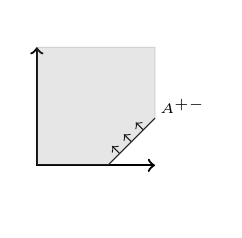
\begin{tikzpicture}[scale=0.5]
\draw [<->,thick] (0.0,3.0) node (yaxis) [above] {}
	|- (3.0,0.0) node (xaxis) [below] {};
\draw (1.8,0.0) -- (3.0,1.2) ;
\draw [->] (2.1,0.3) -- (1.9100000000000001,0.49);
\draw [->] (2.4,0.6) -- (2.21,0.79);
\draw [->] (2.7,0.8999999999999999) -- (2.5100000000000002,1.0899999999999999);
\node at (3.7,1.5) {\tiny $A^{+-}$};
\node at (1.8,-0.9) {\tiny $$};
\draw [fill=gray,opacity=0.2,gray] (1.8,0.0) -- (3.0,1.2) -- (3.0,3.0) -- (0.0,3.0) -- (0.0,0.0) ;
\end{tikzpicture}}
&\hspace{-0.5cm}{\begin{tikzpicture}[scale=0.5]
\draw [<->,thick] (0.0,3.0) node (yaxis) [above] {}
	|- (3.0,0.0) node (xaxis) [below] {};
\draw (1.8,0.0) -- (3.0,1.2) ;
\draw [->] (2.1,0.3) -- (1.9100000000000001,0.49);
\draw [->] (2.4,0.6) -- (2.21,0.79);
\draw [->] (2.7,0.8999999999999999) -- (2.5100000000000002,1.0899999999999999);
\node at (3.7,1.5) {\tiny $A^{+-}$};
\node at (1.8,-0.9) {\tiny $$};
\draw [pattern=north west lines, pattern color=purple] (1.8,0.0) -- (3.0,1.2) -- (3.0,3.0) -- (0.0,3.0) -- (0.0,0.0) ;
\draw (1.8,0.0) -- (3.0,1.2) ;
\draw [->] (2.1,0.3) -- (1.9100000000000001,0.49);
\draw [->] (2.4,0.6) -- (2.21,0.79);
\draw [->] (2.7,0.8999999999999999) -- (2.5100000000000002,1.0899999999999999);
\node at (3.7,1.5) {\tiny $A^{+-}$};
\node at (1.8,-0.9) {\tiny $$};
\draw [pattern=north east lines, pattern color=green!50!black] (3.0,0.0) -- (3.0,3.0) -- (0.0,3.0) -- (0.0,0.0) ;
\end{tikzpicture}}
\\[0pt]
%			\toddText{>n-3}&{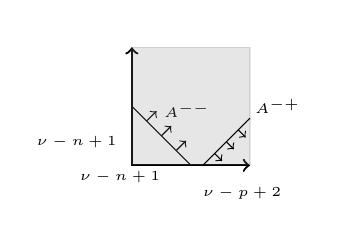
\begin{tikzpicture}[scale=0.5]
\draw [<->,thick] (0.0,3.0) node (yaxis) [above] {}
	|- (3.0,0.0) node (xaxis) [below] {};
\draw (0,1.5)  -- (1.5,0) ;
\draw [->] (0.375,1.125) -- (0.625,1.375);
\draw [->] (0.75,0.75) -- (1.0,1.0);
\draw [->] (1.125,0.375) -- (1.375,0.625);
\node at (-1.4,0.6) {\tiny $\nu-n+1$};
\node at (-0.30000000000000004,-0.3) {\tiny $\nu-n+1$};
\node at (1.4,1.4) {\tiny $A^{--}$};
\draw [fill=gray,opacity=0.2,gray] (3.0,0.0) -- (3.0,3.0) -- (0.0,3.0) -- (0.0,0.0) ;
\draw (1.8,0.0) -- (3.0,1.2) ;
\draw [->] (2.1,0.3) -- (2.29,0.10999999999999999);
\draw [->] (2.4,0.6) -- (2.59,0.41);
\draw [->] (2.7,0.8999999999999999) -- (2.89,0.71);
\node at (3.7,1.5) {\tiny $A^{-+}$};
\node at (2.8,-0.7) {\tiny $\nu-p+2$};
\end{tikzpicture}}
&\hspace{-0.5cm}{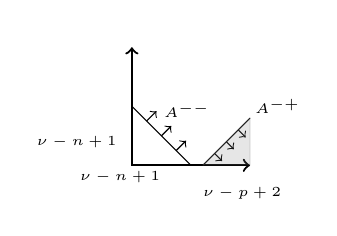
\begin{tikzpicture}[scale=0.5]
\draw [<->,thick] (0.0,3.0) node (yaxis) [above] {}
	|- (3.0,0.0) node (xaxis) [below] {};
\draw (0,1.5)  -- (1.5,0) ;
\draw [->] (0.375,1.125) -- (0.625,1.375);
\draw [->] (0.75,0.75) -- (1.0,1.0);
\draw [->] (1.125,0.375) -- (1.375,0.625);
\node at (-1.4,0.6) {\tiny $\nu-n+1$};
\node at (-0.30000000000000004,-0.3) {\tiny $\nu-n+1$};
\node at (1.4,1.4) {\tiny $A^{--}$};
\draw (1.8,0.0) -- (3.0,1.2) ;
\draw [->] (2.1,0.3) -- (2.29,0.10999999999999999);
\draw [->] (2.4,0.6) -- (2.59,0.41);
\draw [->] (2.7,0.8999999999999999) -- (2.89,0.71);
\node at (3.7,1.5) {\tiny $A^{-+}$};
\node at (2.8,-0.7) {\tiny $\nu-p+2$};
\draw [fill=gray,opacity=0.2,gray] (1.8,0.0) -- (3.0,1.2) -- (3.0,0.0) ;
\end{tikzpicture}}
&\hspace{-0.5cm}{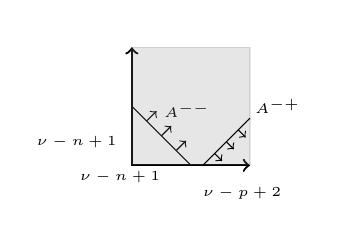
\begin{tikzpicture}[scale=0.5]
\draw [<->,thick] (0.0,3.0) node (yaxis) [above] {}
	|- (3.0,0.0) node (xaxis) [below] {};
\draw (0,1.5)  -- (1.5,0) ;
\draw [->] (0.375,1.125) -- (0.625,1.375);
\draw [->] (0.75,0.75) -- (1.0,1.0);
\draw [->] (1.125,0.375) -- (1.375,0.625);
\node at (-1.4,0.6) {\tiny $\nu-n+1$};
\node at (-0.30000000000000004,-0.3) {\tiny $\nu-n+1$};
\node at (1.4,1.4) {\tiny $A^{--}$};
\draw [fill=gray,opacity=0.2,gray] (3.0,0.0) -- (3.0,3.0) -- (0.0,3.0) -- (0.0,0.0) ;
\draw (1.8,0.0) -- (3.0,1.2) ;
\draw [->] (2.1,0.3) -- (2.29,0.10999999999999999);
\draw [->] (2.4,0.6) -- (2.59,0.41);
\draw [->] (2.7,0.8999999999999999) -- (2.89,0.71);
\node at (3.7,1.5) {\tiny $A^{-+}$};
\node at (2.8,-0.7) {\tiny $\nu-p+2$};
\end{tikzpicture}}
\\[0pt]
%			  
%		\end{tabular}
%		\end{figure}
%	\item Suppose $p,q\in\even$. Then,\clearpage
%		\begin{figure}[h]
%			\noindent\begin{tabular}{m{1.3cm}rrr}
%			$(\lambda,\nu)\in$&$\mybra{\ss\cup\bb}^c$ & $\bb-\ss$  & $\ss-\bb$\\[0pt]
%			\tevenText{\le0}&{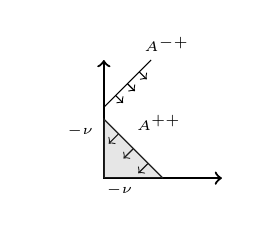
\begin{tikzpicture}[scale=0.5]
\draw [<->,thick] (0.0,3.0) node (yaxis) [above] {}
	|- (3.0,0.0) node (xaxis) [below] {};
\draw (0,1.5)  -- (1.5,0) ;
\draw [->] (0.375,1.125) -- (0.125,0.875);
\draw [->] (0.75,0.75) -- (0.5,0.5);
\draw [->] (1.125,0.375) -- (0.875,0.125);
\node at (1.4,1.4) {\tiny $A^{++}$};
\node at (0.3999999999999999,-0.3) {\tiny $-\nu$};
\node at (-0.6,1.2) {\tiny $-\nu$};
\draw [fill=gray,opacity=0.2,gray] (1.5,0.0) -- (0.0,1.5) -- (0.0,0.0) ;
\draw (0.0,1.8) -- (1.2,3.0) ;
\draw [->] (0.3,2.1) -- (0.49,1.9100000000000001);
\draw [->] (0.6,2.4) -- (0.79,2.21);
\draw [->] (0.8999999999999999,2.7) -- (1.0899999999999999,2.5100000000000002);
\node at (1.6,3.4) {\tiny $A^{-+}$};
\node at (-1.7,1.9000000000000001) {\tiny $$};
\end{tikzpicture}}
&\hspace{-0.5cm}{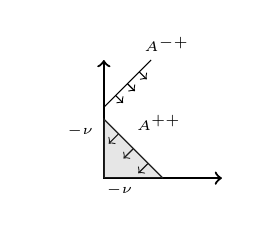
\begin{tikzpicture}[scale=0.5]
\draw [<->,thick] (0.0,3.0) node (yaxis) [above] {}
	|- (3.0,0.0) node (xaxis) [below] {};
\draw (0,1.5)  -- (1.5,0) ;
\draw [->] (0.375,1.125) -- (0.125,0.875);
\draw [->] (0.75,0.75) -- (0.5,0.5);
\draw [->] (1.125,0.375) -- (0.875,0.125);
\node at (1.4,1.4) {\tiny $A^{++}$};
\node at (0.3999999999999999,-0.3) {\tiny $-\nu$};
\node at (-0.6,1.2) {\tiny $-\nu$};
\draw [fill=gray,opacity=0.2,gray] (1.5,0.0) -- (0.0,1.5) -- (0.0,0.0) ;
\draw (0.0,1.8) -- (1.2,3.0) ;
\draw [->] (0.3,2.1) -- (0.49,1.9100000000000001);
\draw [->] (0.6,2.4) -- (0.79,2.21);
\draw [->] (0.8999999999999999,2.7) -- (1.0899999999999999,2.5100000000000002);
\node at (1.6,3.4) {\tiny $A^{-+}$};
\node at (-1.7,1.9000000000000001) {\tiny $$};
\end{tikzpicture}}
&\hspace{-0.5cm}{\begin{tikzpicture}[scale=0.5]
\draw [<->,thick] (0.0,3.0) node (yaxis) [above] {}
	|- (3.0,0.0) node (xaxis) [below] {};
\draw (0,1.5)  -- (1.5,0) ;
\draw [->] (0.375,1.125) -- (0.125,0.875);
\draw [->] (0.75,0.75) -- (0.5,0.5);
\draw [->] (1.125,0.375) -- (0.875,0.125);
\node at (1.4,1.4) {\tiny $A^{++}$};
\node at (0.3999999999999999,-0.3) {\tiny $-\nu$};
\node at (-0.6,1.2) {\tiny $-\nu$};
\draw [pattern=north west lines, pattern color=purple] (1.5,0.0) -- (0.0,1.5) -- (0.0,0.0) ;
\draw (0.0,1.8) -- (1.2,3.0) ;
\draw [->] (0.3,2.1) -- (0.49,1.9100000000000001);
\draw [->] (0.6,2.4) -- (0.79,2.21);
\draw [->] (0.8999999999999999,2.7) -- (1.0899999999999999,2.5100000000000002);
\node at (1.6,3.4) {\tiny $A^{-+}$};
\node at (-1.7,1.9000000000000001) {\tiny $$};
\draw [pattern=north east lines, pattern color=green!50!black] (3.0,0.0) -- (3.0,3.0) -- (0.0,3.0) -- (0.0,0.0) ;
\end{tikzpicture}}
\\[0pt]
%			\toddText{\le n-3}&{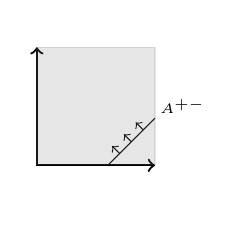
\begin{tikzpicture}[scale=0.5]
\draw [<->,thick] (0.0,3.0) node (yaxis) [above] {}
	|- (3.0,0.0) node (xaxis) [below] {};
\draw (1.8,0.0) -- (3.0,1.2) ;
\draw [->] (2.1,0.3) -- (1.9100000000000001,0.49);
\draw [->] (2.4,0.6) -- (2.21,0.79);
\draw [->] (2.7,0.8999999999999999) -- (2.5100000000000002,1.0899999999999999);
\node at (3.7,1.5) {\tiny $A^{+-}$};
\node at (1.8,-0.9) {\tiny $$};
\draw [fill=gray,opacity=0.2,gray] (3.0,0.0) -- (3.0,3.0) -- (0.0,3.0) -- (0.0,0.0) ;
\end{tikzpicture}}
&\hspace{-0.5cm}{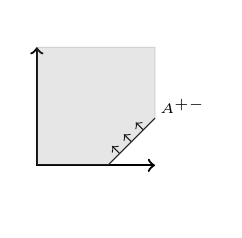
\begin{tikzpicture}[scale=0.5]
\draw [<->,thick] (0.0,3.0) node (yaxis) [above] {}
	|- (3.0,0.0) node (xaxis) [below] {};
\draw (1.8,0.0) -- (3.0,1.2) ;
\draw [->] (2.1,0.3) -- (1.9100000000000001,0.49);
\draw [->] (2.4,0.6) -- (2.21,0.79);
\draw [->] (2.7,0.8999999999999999) -- (2.5100000000000002,1.0899999999999999);
\node at (3.7,1.5) {\tiny $A^{+-}$};
\node at (1.8,-0.9) {\tiny $$};
\draw [fill=gray,opacity=0.2,gray] (1.8,0.0) -- (3.0,1.2) -- (3.0,3.0) -- (0.0,3.0) -- (0.0,0.0) ;
\end{tikzpicture}}
&\hspace{-0.5cm}{\begin{tikzpicture}[scale=0.5]
\draw [<->,thick] (0.0,3.0) node (yaxis) [above] {}
	|- (3.0,0.0) node (xaxis) [below] {};
\draw (1.8,0.0) -- (3.0,1.2) ;
\draw [->] (2.1,0.3) -- (1.9100000000000001,0.49);
\draw [->] (2.4,0.6) -- (2.21,0.79);
\draw [->] (2.7,0.8999999999999999) -- (2.5100000000000002,1.0899999999999999);
\node at (3.7,1.5) {\tiny $A^{+-}$};
\node at (1.8,-0.9) {\tiny $$};
\draw [pattern=north east lines, pattern color=green!50!black] (3.0,0.0) -- (3.0,3.0) -- (0.0,3.0) -- (0.0,0.0) ;
\draw (1.8,0.0) -- (3.0,1.2) ;
\draw [->] (2.1,0.3) -- (1.9100000000000001,0.49);
\draw [->] (2.4,0.6) -- (2.21,0.79);
\draw [->] (2.7,0.8999999999999999) -- (2.5100000000000002,1.0899999999999999);
\node at (3.7,1.5) {\tiny $A^{+-}$};
\node at (1.8,-0.9) {\tiny $$};
\draw [pattern=north west lines, pattern color=purple] (1.8,0.0) -- (3.0,1.2) -- (3.0,3.0) -- (0.0,3.0) -- (0.0,0.0) ;
\end{tikzpicture}}
\\[0pt]
%			\tevenText{>0}&{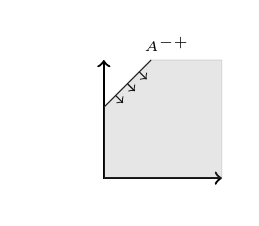
\begin{tikzpicture}[scale=0.5]
\draw [<->,thick] (0.0,3.0) node (yaxis) [above] {}
	|- (3.0,0.0) node (xaxis) [below] {};
\draw (0.0,1.8) -- (1.2,3.0) ;
\draw [->] (0.3,2.1) -- (0.49,1.9100000000000001);
\draw [->] (0.6,2.4) -- (0.79,2.21);
\draw [->] (0.8999999999999999,2.7) -- (1.0899999999999999,2.5100000000000002);
\node at (1.6,3.4) {\tiny $A^{-+}$};
\node at (-1.7,1.9000000000000001) {\tiny $$};
\draw [fill=gray,opacity=0.2,gray] (0.0,1.8) -- (1.2,3.0) -- (3.0,3.0) -- (3.0,0.0) -- (0.0,0.0) ;
\end{tikzpicture}}
&\hspace{-0.5cm}{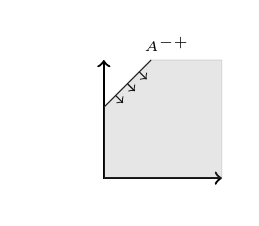
\begin{tikzpicture}[scale=0.5]
\draw [<->,thick] (0.0,3.0) node (yaxis) [above] {}
	|- (3.0,0.0) node (xaxis) [below] {};
\draw (0.0,1.8) -- (1.2,3.0) ;
\draw [->] (0.3,2.1) -- (0.49,1.9100000000000001);
\draw [->] (0.6,2.4) -- (0.79,2.21);
\draw [->] (0.8999999999999999,2.7) -- (1.0899999999999999,2.5100000000000002);
\node at (1.6,3.4) {\tiny $A^{-+}$};
\node at (-1.7,1.9000000000000001) {\tiny $$};
\draw [fill=gray,opacity=0.2,gray] (0.0,1.8) -- (1.2,3.0) -- (3.0,3.0) -- (3.0,0.0) -- (0.0,0.0) ;
\end{tikzpicture}}
&\hspace{-0.5cm}{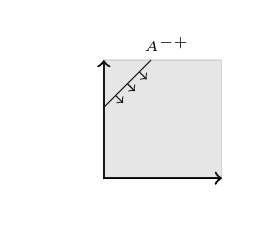
\begin{tikzpicture}[scale=0.5]
\draw [<->,thick] (0.0,3.0) node (yaxis) [above] {}
	|- (3.0,0.0) node (xaxis) [below] {};
\draw (0.0,1.8) -- (1.2,3.0) ;
\draw [->] (0.3,2.1) -- (0.49,1.9100000000000001);
\draw [->] (0.6,2.4) -- (0.79,2.21);
\draw [->] (0.8999999999999999,2.7) -- (1.0899999999999999,2.5100000000000002);
\node at (1.6,3.4) {\tiny $A^{-+}$};
\node at (-1.7,1.9000000000000001) {\tiny $$};
\draw [fill=gray,opacity=0.2,gray] (3.0,0.0) -- (3.0,3.0) -- (0.0,3.0) -- (0.0,0.0) ;
\end{tikzpicture}}
\\[0pt]
%			\toddText{>n-3}&{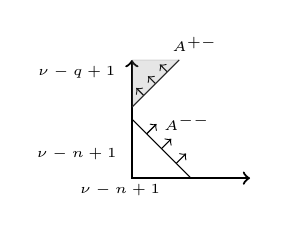
\begin{tikzpicture}[scale=0.5]
\draw [<->,thick] (0.0,3.0) node (yaxis) [above] {}
	|- (3.0,0.0) node (xaxis) [below] {};
\draw (0,1.5)  -- (1.5,0) ;
\draw [->] (0.375,1.125) -- (0.625,1.375);
\draw [->] (0.75,0.75) -- (1.0,1.0);
\draw [->] (1.125,0.375) -- (1.375,0.625);
\node at (-1.4,0.6) {\tiny $\nu-n+1$};
\node at (-0.30000000000000004,-0.3) {\tiny $\nu-n+1$};
\node at (1.4,1.4) {\tiny $A^{--}$};
\draw (0.0,1.8) -- (1.2,3.0) ;
\draw [->] (0.3,2.1) -- (0.10999999999999999,2.29);
\draw [->] (0.6,2.4) -- (0.41,2.59);
\draw [->] (0.8999999999999999,2.7) -- (0.71,2.89);
\node at (1.6,3.4) {\tiny $A^{+-}$};
\node at (-1.4,2.7) {\tiny $\nu-q+1$};
\draw [fill=gray,opacity=0.2,gray] (0.0,1.8) -- (1.2,3.0) -- (0.0,3.0) ;
\end{tikzpicture}}
&\hspace{-0.5cm}{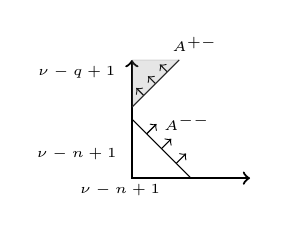
\begin{tikzpicture}[scale=0.5]
\draw [<->,thick] (0.0,3.0) node (yaxis) [above] {}
	|- (3.0,0.0) node (xaxis) [below] {};
\draw (0,1.5)  -- (1.5,0) ;
\draw [->] (0.375,1.125) -- (0.625,1.375);
\draw [->] (0.75,0.75) -- (1.0,1.0);
\draw [->] (1.125,0.375) -- (1.375,0.625);
\node at (-1.4,0.6) {\tiny $\nu-n+1$};
\node at (-0.30000000000000004,-0.3) {\tiny $\nu-n+1$};
\node at (1.4,1.4) {\tiny $A^{--}$};
\draw (0.0,1.8) -- (1.2,3.0) ;
\draw [->] (0.3,2.1) -- (0.10999999999999999,2.29);
\draw [->] (0.6,2.4) -- (0.41,2.59);
\draw [->] (0.8999999999999999,2.7) -- (0.71,2.89);
\node at (1.6,3.4) {\tiny $A^{+-}$};
\node at (-1.4,2.7) {\tiny $\nu-q+1$};
\draw [fill=gray,opacity=0.2,gray] (0.0,1.8) -- (1.2,3.0) -- (0.0,3.0) ;
\end{tikzpicture}}
&\hspace{-0.5cm}{\begin{tikzpicture}[scale=0.5]
\draw [<->,thick] (0.0,3.0) node (yaxis) [above] {}
	|- (3.0,0.0) node (xaxis) [below] {};
\draw (0,1.5)  -- (1.5,0) ;
\draw [->] (0.375,1.125) -- (0.625,1.375);
\draw [->] (0.75,0.75) -- (1.0,1.0);
\draw [->] (1.125,0.375) -- (1.375,0.625);
\node at (-1.4,0.6) {\tiny $\nu-n+1$};
\node at (-0.30000000000000004,-0.3) {\tiny $\nu-n+1$};
\node at (1.4,1.4) {\tiny $A^{--}$};
\draw [pattern=north east lines, pattern color=green!50!black] (3.0,0.0) -- (3.0,3.0) -- (0.0,3.0) -- (0.0,0.0) ;
\draw (0.0,1.8) -- (1.2,3.0) ;
\draw [->] (0.3,2.1) -- (0.10999999999999999,2.29);
\draw [->] (0.6,2.4) -- (0.41,2.59);
\draw [->] (0.8999999999999999,2.7) -- (0.71,2.89);
\node at (1.6,3.4) {\tiny $A^{+-}$};
\node at (-1.4,2.7) {\tiny $\nu-q+1$};
\draw [pattern=north west lines, pattern color=purple] (0.0,1.8) -- (1.2,3.0) -- (0.0,3.0) ;
\end{tikzpicture}}
\\[0pt]
%		\end{tabular}
%		\end{figure}
%	\item Suppose $p\in\even,q\in\odd$. Then for $\nu\in\odd$, $R_{\lambda,\nu}^X$ is surjective. Otherwise (for $\nu\in\even$) we have,\clearpage
%	  \begin{figure}[h]
%		  \noindent\begin{tabular}{@{}m{1.6cm}@{}ccc}
%	      $(\lambda,\nu)\in$&$\mybra{//\cup\backslash\backslash}^c$ & $\backslash\backslash-//$  & $//\cap\backslash\backslash,k> l$\\[0pt]
%	      \vspace{-3cm}$\nu\leq0$&{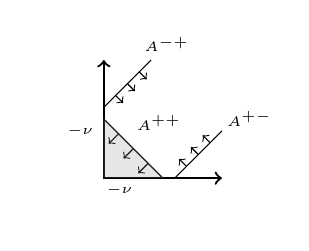
\begin{tikzpicture}[scale=0.5]
\draw [<->,thick] (0.0,3.0) node (yaxis) [above] {}
	|- (3.0,0.0) node (xaxis) [below] {};
\draw (0,1.5)  -- (1.5,0) ;
\draw [->] (0.375,1.125) -- (0.125,0.875);
\draw [->] (0.75,0.75) -- (0.5,0.5);
\draw [->] (1.125,0.375) -- (0.875,0.125);
\node at (1.4,1.4) {\tiny $A^{++}$};
\node at (0.3999999999999999,-0.3) {\tiny $-\nu$};
\node at (-0.6,1.2) {\tiny $-\nu$};
\draw [fill=gray,opacity=0.2,gray] (1.5,0.0) -- (0.0,1.5) -- (0.0,0.0) ;
\draw (1.8,0.0) -- (3.0,1.2) ;
\draw [->] (2.1,0.3) -- (1.9100000000000001,0.49);
\draw [->] (2.4,0.6) -- (2.21,0.79);
\draw [->] (2.7,0.8999999999999999) -- (2.5100000000000002,1.0899999999999999);
\node at (3.7,1.5) {\tiny $A^{+-}$};
\node at (1.8,-0.9) {\tiny $$};
\draw (0.0,1.8) -- (1.2,3.0) ;
\draw [->] (0.3,2.1) -- (0.49,1.9100000000000001);
\draw [->] (0.6,2.4) -- (0.79,2.21);
\draw [->] (0.8999999999999999,2.7) -- (1.0899999999999999,2.5100000000000002);
\node at (1.6,3.4) {\tiny $A^{-+}$};
\node at (-1.7,1.9000000000000001) {\tiny $$};
\end{tikzpicture}}
&\hspace{-0.5cm}{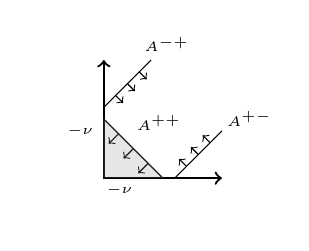
\begin{tikzpicture}[scale=0.5]
\draw [<->,thick] (0.0,3.0) node (yaxis) [above] {}
	|- (3.0,0.0) node (xaxis) [below] {};
\draw (0,1.5)  -- (1.5,0) ;
\draw [->] (0.375,1.125) -- (0.125,0.875);
\draw [->] (0.75,0.75) -- (0.5,0.5);
\draw [->] (1.125,0.375) -- (0.875,0.125);
\node at (1.4,1.4) {\tiny $A^{++}$};
\node at (0.3999999999999999,-0.3) {\tiny $-\nu$};
\node at (-0.6,1.2) {\tiny $-\nu$};
\draw [fill=gray,opacity=0.2,gray] (1.5,0.0) -- (0.0,1.5) -- (0.0,0.0) ;
\draw (1.8,0.0) -- (3.0,1.2) ;
\draw [->] (2.1,0.3) -- (1.9100000000000001,0.49);
\draw [->] (2.4,0.6) -- (2.21,0.79);
\draw [->] (2.7,0.8999999999999999) -- (2.5100000000000002,1.0899999999999999);
\node at (3.7,1.5) {\tiny $A^{+-}$};
\node at (1.8,-0.9) {\tiny $$};
\draw (0.0,1.8) -- (1.2,3.0) ;
\draw [->] (0.3,2.1) -- (0.49,1.9100000000000001);
\draw [->] (0.6,2.4) -- (0.79,2.21);
\draw [->] (0.8999999999999999,2.7) -- (1.0899999999999999,2.5100000000000002);
\node at (1.6,3.4) {\tiny $A^{-+}$};
\node at (-1.7,1.9000000000000001) {\tiny $$};
\end{tikzpicture}}
&\hspace{-0.5cm}{\begin{tikzpicture}[scale=0.5]
\draw [<->,thick] (0.0,3.0) node (yaxis) [above] {}
	|- (3.0,0.0) node (xaxis) [below] {};
\draw (0,1.5)  -- (1.5,0) ;
\draw [->] (0.375,1.125) -- (0.125,0.875);
\draw [->] (0.75,0.75) -- (0.5,0.5);
\draw [->] (1.125,0.375) -- (0.875,0.125);
\node at (1.4,1.4) {\tiny $A^{++}$};
\node at (0.3999999999999999,-0.3) {\tiny $-\nu$};
\node at (-0.6,1.2) {\tiny $-\nu$};
\draw [pattern=north west lines, pattern color=purple] (1.5,0.0) -- (0.0,1.5) -- (0.0,0.0) ;
\draw (1.8,0.0) -- (3.0,1.2) ;
\draw [->] (2.1,0.3) -- (1.9100000000000001,0.49);
\draw [->] (2.4,0.6) -- (2.21,0.79);
\draw [->] (2.7,0.8999999999999999) -- (2.5100000000000002,1.0899999999999999);
\node at (3.7,1.5) {\tiny $A^{+-}$};
\node at (1.8,-0.9) {\tiny $$};
\draw [pattern=north east lines, pattern color=green!50!black] (3.0,0.0) -- (3.0,3.0) -- (0.0,3.0) -- (0.0,0.0) ;
\draw (0.0,1.8) -- (1.2,3.0) ;
\draw [->] (0.3,2.1) -- (0.49,1.9100000000000001);
\draw [->] (0.6,2.4) -- (0.79,2.21);
\draw [->] (0.8999999999999999,2.7) -- (1.0899999999999999,2.5100000000000002);
\node at (1.6,3.4) {\tiny $A^{-+}$};
\node at (-1.7,1.9000000000000001) {\tiny $$};
\end{tikzpicture}}
\\[0pt]
%	      \vspace{-3cm}$
%	      \begin{array}{l}
%		      \nu>0\\\nu\le\frac{n-3}{2}
%	      \end{array}
%	      $&{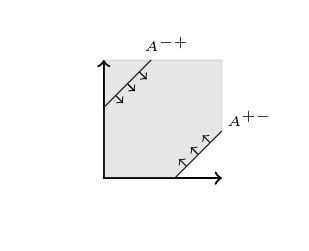
\begin{tikzpicture}[scale=0.5]
\draw [<->,thick] (0.0,3.0) node (yaxis) [above] {}
	|- (3.0,0.0) node (xaxis) [below] {};
\draw (1.8,0.0) -- (3.0,1.2) ;
\draw [->] (2.1,0.3) -- (1.9100000000000001,0.49);
\draw [->] (2.4,0.6) -- (2.21,0.79);
\draw [->] (2.7,0.8999999999999999) -- (2.5100000000000002,1.0899999999999999);
\node at (3.7,1.5) {\tiny $A^{+-}$};
\node at (1.8,-0.9) {\tiny $$};
\draw [fill=gray,opacity=0.2,gray] (1.8,0.0) -- (3.0,1.2) -- (3.0,3.0) -- (1.2,3.0) -- (0.0,1.8) -- (0.0,0.0) ;
\draw (0.0,1.8) -- (1.2,3.0) ;
\draw [->] (0.3,2.1) -- (0.49,1.9100000000000001);
\draw [->] (0.6,2.4) -- (0.79,2.21);
\draw [->] (0.8999999999999999,2.7) -- (1.0899999999999999,2.5100000000000002);
\node at (1.6,3.4) {\tiny $A^{-+}$};
\node at (-1.7,1.9000000000000001) {\tiny $$};
\draw [fill=gray,opacity=0.2,gray] (0.0,1.8) -- (1.2,3.0) -- (0.0,3.0) ;
\end{tikzpicture}}
&\hspace{-0.5cm}{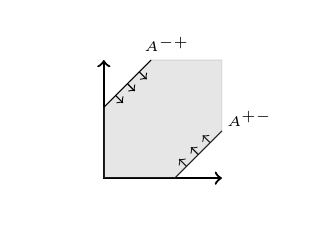
\begin{tikzpicture}[scale=0.5]
\draw [<->,thick] (0.0,3.0) node (yaxis) [above] {}
	|- (3.0,0.0) node (xaxis) [below] {};
\draw (1.8,0.0) -- (3.0,1.2) ;
\draw [->] (2.1,0.3) -- (1.9100000000000001,0.49);
\draw [->] (2.4,0.6) -- (2.21,0.79);
\draw [->] (2.7,0.8999999999999999) -- (2.5100000000000002,1.0899999999999999);
\node at (3.7,1.5) {\tiny $A^{+-}$};
\node at (1.8,-0.9) {\tiny $$};
\draw [fill=gray,opacity=0.2,gray] (1.8,0.0) -- (3.0,1.2) -- (3.0,3.0) -- (1.2,3.0) -- (0.0,1.8) -- (0.0,0.0) ;
\draw (0.0,1.8) -- (1.2,3.0) ;
\draw [->] (0.3,2.1) -- (0.49,1.9100000000000001);
\draw [->] (0.6,2.4) -- (0.79,2.21);
\draw [->] (0.8999999999999999,2.7) -- (1.0899999999999999,2.5100000000000002);
\node at (1.6,3.4) {\tiny $A^{-+}$};
\node at (-1.7,1.9000000000000001) {\tiny $$};
\end{tikzpicture}}
&\hspace{-0.5cm}{\begin{tikzpicture}[scale=0.5]
\draw [<->,thick] (0.0,3.0) node (yaxis) [above] {}
	|- (3.0,0.0) node (xaxis) [below] {};
\draw (1.8,0.0) -- (3.0,1.2) ;
\draw [->] (2.1,0.3) -- (1.9100000000000001,0.49);
\draw [->] (2.4,0.6) -- (2.21,0.79);
\draw [->] (2.7,0.8999999999999999) -- (2.5100000000000002,1.0899999999999999);
\node at (3.7,1.5) {\tiny $A^{+-}$};
\node at (1.8,-0.9) {\tiny $$};
\draw [pattern=north west lines, pattern color=purple] (1.8,0.0) -- (3.0,1.2) -- (3.0,3.0) -- (0.0,3.0) -- (0.0,0.0) ;
\draw (0.0,1.8) -- (1.2,3.0) ;
\draw [->] (0.3,2.1) -- (0.49,1.9100000000000001);
\draw [->] (0.6,2.4) -- (0.79,2.21);
\draw [->] (0.8999999999999999,2.7) -- (1.0899999999999999,2.5100000000000002);
\node at (1.6,3.4) {\tiny $A^{-+}$};
\node at (-1.7,1.9000000000000001) {\tiny $$};
\draw [pattern=north east lines, pattern color=green!50!black] (3.0,0.0) -- (3.0,3.0) -- (0.0,3.0) -- (0.0,0.0) ;
\end{tikzpicture}}
\\[0pt]
%              $(\lambda,\nu)\in$&$\mybra{//\cup\backslash\backslash}^c$ && $//\cap\backslash\backslash,k=l$\\[0pt]
%	      \vspace{-3cm}$
%	      \begin{array}{l}
%		      \nu\todd\\\nu=\frac{n-1}{2}
%	      \end{array}
%	      $&{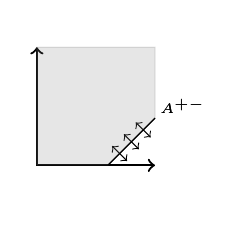
\begin{tikzpicture}[scale=0.5]
\draw [<->,thick] (0.0,3.0) node (yaxis) [above] {}
	|- (3.0,0.0) node (xaxis) [below] {};
\draw (1.8,0.0) -- (3.0,1.2) ;
\draw [->] (2.1,0.3) -- (1.9100000000000001,0.49);
\draw [->] (2.4,0.6) -- (2.21,0.79);
\draw [->] (2.7,0.8999999999999999) -- (2.5100000000000002,1.0899999999999999);
\node at (3.7,1.5) {\tiny $A^{+-}$};
\node at (1.8,-0.9) {\tiny $$};
\draw [fill=gray,opacity=0.2,gray] (1.8,0.0) -- (3.0,1.2) -- (3.0,3.0) -- (0.0,3.0) -- (0.0,0.0) ;
\draw (1.8,0.0) -- (3.0,1.2) ;
\draw [->] (2.1,0.3) -- (2.29,0.10999999999999999);
\draw [->] (2.4,0.6) -- (2.59,0.41);
\draw [->] (2.7,0.8999999999999999) -- (2.89,0.71);
\node at (3.7,1.5) {\tiny $A^{+-}$};
\node at (1.8,-0.9) {\tiny $$};
\end{tikzpicture}}
&\hspace{-0.5cm}&\hspace{-0.5cm}{\begin{tikzpicture}[scale=0.5]
\draw [<->,thick] (0.0,3.0) node (yaxis) [above] {}
	|- (3.0,0.0) node (xaxis) [below] {};
\draw (1.8,0.0) -- (3.0,1.2) ;
\draw [->] (2.1,0.3) -- (1.9100000000000001,0.49);
\draw [->] (2.4,0.6) -- (2.21,0.79);
\draw [->] (2.7,0.8999999999999999) -- (2.5100000000000002,1.0899999999999999);
\node at (3.7,1.5) {\tiny $A^{+-}$};
\node at (1.8,-0.9) {\tiny $$};
\draw [pattern=north west lines, pattern color=purple] (1.8,0.0) -- (3.0,1.2) -- (3.0,3.0) -- (0.0,3.0) -- (0.0,0.0) ;
\draw (1.8,0.0) -- (3.0,1.2) ;
\draw [->] (2.1,0.3) -- (2.29,0.10999999999999999);
\draw [->] (2.4,0.6) -- (2.59,0.41);
\draw [->] (2.7,0.8999999999999999) -- (2.89,0.71);
\node at (3.7,1.5) {\tiny $A^{+-}$};
\node at (1.8,-0.9) {\tiny $$};
\draw [pattern=north east lines, pattern color=green!50!black] (3.0,0.0) -- (3.0,3.0) -- (0.0,3.0) -- (0.0,0.0) ;
\end{tikzpicture}}
\\[0pt]
%	      $(\lambda,\nu)\in$&$\mybra{//\cup\backslash\backslash}^c$ & $//-\backslash\backslash$  & $//\cap\backslash\backslash,k< l$\\[0pt]
%	      \vspace{-3cm}
%	      $
%	      \begin{array}{l}
%		      \nu\ge\frac{n+1}{2}\\\nu\le n-3
%	      \end{array}
%	      $
%	      &{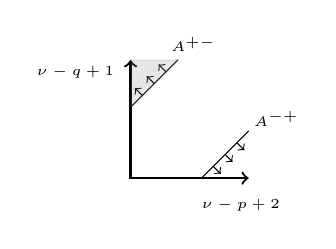
\begin{tikzpicture}[scale=0.5]
\draw [<->,thick] (0.0,3.0) node (yaxis) [above] {}
	|- (3.0,0.0) node (xaxis) [below] {};
\draw (1.8,0.0) -- (3.0,1.2) ;
\draw [->] (2.1,0.3) -- (2.29,0.10999999999999999);
\draw [->] (2.4,0.6) -- (2.59,0.41);
\draw [->] (2.7,0.8999999999999999) -- (2.89,0.71);
\node at (3.7,1.5) {\tiny $A^{-+}$};
\node at (2.8,-0.7) {\tiny $\nu-p+2$};
\draw (0.0,1.8) -- (1.2,3.0) ;
\draw [->] (0.3,2.1) -- (0.10999999999999999,2.29);
\draw [->] (0.6,2.4) -- (0.41,2.59);
\draw [->] (0.8999999999999999,2.7) -- (0.71,2.89);
\node at (1.6,3.4) {\tiny $A^{+-}$};
\node at (-1.4,2.7) {\tiny $\nu-q+1$};
\draw [fill=gray,opacity=0.2,gray] (0.0,1.8) -- (1.2,3.0) -- (0.0,3.0) ;
\end{tikzpicture}}
&\hspace{-0.5cm}{\begin{tikzpicture}[scale=0.5]
\draw [<->,thick] (0.0,3.0) node (yaxis) [above] {}
	|- (3.0,0.0) node (xaxis) [below] {};
\draw (1.8,0.0) -- (3.0,1.2) ;
\draw [->] (2.1,0.3) -- (2.29,0.10999999999999999);
\draw [->] (2.4,0.6) -- (2.59,0.41);
\draw [->] (2.7,0.8999999999999999) -- (2.89,0.71);
\node at (3.7,1.5) {\tiny $A^{-+}$};
\node at (2.8,-0.7) {\tiny $\nu-p+2$};
\draw [pattern=north east lines, pattern color=green!50!black] (3.0,0.0) -- (3.0,3.0) -- (0.0,3.0) -- (0.0,0.0) ;
\draw (0.0,1.8) -- (1.2,3.0) ;
\draw [->] (0.3,2.1) -- (0.10999999999999999,2.29);
\draw [->] (0.6,2.4) -- (0.41,2.59);
\draw [->] (0.8999999999999999,2.7) -- (0.71,2.89);
\node at (1.6,3.4) {\tiny $A^{+-}$};
\node at (-1.4,2.7) {\tiny $\nu-q+1$};
\draw [pattern=north west lines, pattern color=purple] (0.0,1.8) -- (1.2,3.0) -- (0.0,3.0) ;
\end{tikzpicture}}
&\hspace{-0.5cm}{\begin{tikzpicture}[scale=0.5]
\draw [<->,thick] (0.0,3.0) node (yaxis) [above] {}
	|- (3.0,0.0) node (xaxis) [below] {};
\draw (1.8,0.0) -- (3.0,1.2) ;
\draw [->] (2.1,0.3) -- (2.29,0.10999999999999999);
\draw [->] (2.4,0.6) -- (2.59,0.41);
\draw [->] (2.7,0.8999999999999999) -- (2.89,0.71);
\node at (3.7,1.5) {\tiny $A^{-+}$};
\node at (2.8,-0.7) {\tiny $\nu-p+2$};
\draw [pattern=north east lines, pattern color=green!50!black] (1.8,0.0) -- (3.0,1.2) -- (3.0,0.0) ;
\draw (0.0,1.8) -- (1.2,3.0) ;
\draw [->] (0.3,2.1) -- (0.10999999999999999,2.29);
\draw [->] (0.6,2.4) -- (0.41,2.59);
\draw [->] (0.8999999999999999,2.7) -- (0.71,2.89);
\node at (1.6,3.4) {\tiny $A^{+-}$};
\node at (-1.4,2.7) {\tiny $\nu-q+1$};
\draw [pattern=north west lines, pattern color=purple] (0.0,1.8) -- (1.2,3.0) -- (0.0,3.0) ;
\draw (0.0,1.8) -- (1.2,3.0) ;
\draw [->] (0.3,2.1) -- (0.10999999999999999,2.29);
\draw [->] (0.6,2.4) -- (0.41,2.59);
\draw [->] (0.8999999999999999,2.7) -- (0.71,2.89);
\node at (1.6,3.4) {\tiny $A^{+-}$};
\node at (-1.4,2.7) {\tiny $\nu-q+1$};
\draw [pattern=north east lines, pattern color=green!50!black] (0.0,1.8) -- (1.2,3.0) -- (0.0,3.0) ;
\end{tikzpicture}}
\\[0pt]
%	      \vspace{-3cm}$
%	      \nu>n-3$&{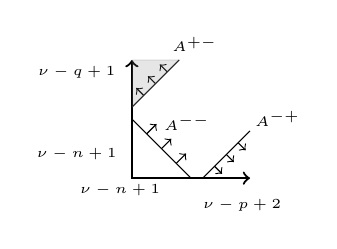
\begin{tikzpicture}[scale=0.5]
\draw [<->,thick] (0.0,3.0) node (yaxis) [above] {}
	|- (3.0,0.0) node (xaxis) [below] {};
\draw (0,1.5)  -- (1.5,0) ;
\draw [->] (0.375,1.125) -- (0.625,1.375);
\draw [->] (0.75,0.75) -- (1.0,1.0);
\draw [->] (1.125,0.375) -- (1.375,0.625);
\node at (-1.4,0.6) {\tiny $\nu-n+1$};
\node at (-0.30000000000000004,-0.3) {\tiny $\nu-n+1$};
\node at (1.4,1.4) {\tiny $A^{--}$};
\draw (1.8,0.0) -- (3.0,1.2) ;
\draw [->] (2.1,0.3) -- (2.29,0.10999999999999999);
\draw [->] (2.4,0.6) -- (2.59,0.41);
\draw [->] (2.7,0.8999999999999999) -- (2.89,0.71);
\node at (3.7,1.5) {\tiny $A^{-+}$};
\node at (2.8,-0.7) {\tiny $\nu-p+2$};
\draw (0.0,1.8) -- (1.2,3.0) ;
\draw [->] (0.3,2.1) -- (0.10999999999999999,2.29);
\draw [->] (0.6,2.4) -- (0.41,2.59);
\draw [->] (0.8999999999999999,2.7) -- (0.71,2.89);
\node at (1.6,3.4) {\tiny $A^{+-}$};
\node at (-1.4,2.7) {\tiny $\nu-q+1$};
\draw [fill=gray,opacity=0.2,gray] (0.0,1.8) -- (1.2,3.0) -- (0.0,3.0) ;
\end{tikzpicture}}
&\hspace{-0.5cm}{\begin{tikzpicture}[scale=0.5]
\draw [<->,thick] (0.0,3.0) node (yaxis) [above] {}
	|- (3.0,0.0) node (xaxis) [below] {};
\draw (0,1.5)  -- (1.5,0) ;
\draw [->] (0.375,1.125) -- (0.625,1.375);
\draw [->] (0.75,0.75) -- (1.0,1.0);
\draw [->] (1.125,0.375) -- (1.375,0.625);
\node at (-1.4,0.6) {\tiny $\nu-n+1$};
\node at (-0.30000000000000004,-0.3) {\tiny $\nu-n+1$};
\node at (1.4,1.4) {\tiny $A^{--}$};
\draw (1.8,0.0) -- (3.0,1.2) ;
\draw [->] (2.1,0.3) -- (2.29,0.10999999999999999);
\draw [->] (2.4,0.6) -- (2.59,0.41);
\draw [->] (2.7,0.8999999999999999) -- (2.89,0.71);
\node at (3.7,1.5) {\tiny $A^{-+}$};
\node at (2.8,-0.7) {\tiny $\nu-p+2$};
\draw [pattern=north east lines, pattern color=green!50!black] (3.0,0.0) -- (3.0,3.0) -- (0.0,3.0) -- (0.0,0.0) ;
\draw (0.0,1.8) -- (1.2,3.0) ;
\draw [->] (0.3,2.1) -- (0.10999999999999999,2.29);
\draw [->] (0.6,2.4) -- (0.41,2.59);
\draw [->] (0.8999999999999999,2.7) -- (0.71,2.89);
\node at (1.6,3.4) {\tiny $A^{+-}$};
\node at (-1.4,2.7) {\tiny $\nu-q+1$};
\draw [pattern=north west lines, pattern color=purple] (0.0,1.8) -- (1.2,3.0) -- (0.0,3.0) ;
\end{tikzpicture}}
&\hspace{-0.5cm}{\begin{tikzpicture}[scale=0.5]
\draw [<->,thick] (0.0,3.0) node (yaxis) [above] {}
	|- (3.0,0.0) node (xaxis) [below] {};
\draw (0,1.5)  -- (1.5,0) ;
\draw [->] (0.375,1.125) -- (0.625,1.375);
\draw [->] (0.75,0.75) -- (1.0,1.0);
\draw [->] (1.125,0.375) -- (1.375,0.625);
\node at (-1.4,0.6) {\tiny $\nu-n+1$};
\node at (-0.30000000000000004,-0.3) {\tiny $\nu-n+1$};
\node at (1.4,1.4) {\tiny $A^{--}$};
\draw (1.8,0.0) -- (3.0,1.2) ;
\draw [->] (2.1,0.3) -- (2.29,0.10999999999999999);
\draw [->] (2.4,0.6) -- (2.59,0.41);
\draw [->] (2.7,0.8999999999999999) -- (2.89,0.71);
\node at (3.7,1.5) {\tiny $A^{-+}$};
\node at (2.8,-0.7) {\tiny $\nu-p+2$};
\draw [pattern=north east lines, pattern color=green!50!black] (1.8,0.0) -- (3.0,1.2) -- (3.0,0.0) ;
\draw (0.0,1.8) -- (1.2,3.0) ;
\draw [->] (0.3,2.1) -- (0.10999999999999999,2.29);
\draw [->] (0.6,2.4) -- (0.41,2.59);
\draw [->] (0.8999999999999999,2.7) -- (0.71,2.89);
\node at (1.6,3.4) {\tiny $A^{+-}$};
\node at (-1.4,2.7) {\tiny $\nu-q+1$};
\draw [pattern=north west lines, pattern color=purple] (0.0,1.8) -- (1.2,3.0) -- (0.0,3.0) ;
\draw (0.0,1.8) -- (1.2,3.0) ;
\draw [->] (0.3,2.1) -- (0.10999999999999999,2.29);
\draw [->] (0.6,2.4) -- (0.41,2.59);
\draw [->] (0.8999999999999999,2.7) -- (0.71,2.89);
\node at (1.6,3.4) {\tiny $A^{+-}$};
\node at (-1.4,2.7) {\tiny $\nu-q+1$};
\draw [pattern=north east lines, pattern color=green!50!black] (0.0,1.8) -- (1.2,3.0) -- (0.0,3.0) ;
\end{tikzpicture}}
\\[0pt]
%	    \end{tabular}
%	  \end{figure}
%	\end{enumerate}
%	\vspace{-0.9cm}
%	In the diagrams above some of them are filled not with gray, but with colored diagonal lines. This means that the image of the regular
%	SBO $R_{\lambda,\nu}^X$ is zero and the (green/purple)
%	ascending/descending diagonal lines show the images of its residues $R_{\lambda,\nu}^{ \left\{ o \right\}}$ and $\tilde{R}_{\lambda,\nu}^X$ respectively.
%
%	For $p=1$ we have:\clearpage
%
%	\begin{figure}[h]
%		\begin{tabular}{p{4.1cm}p{2.0cm}p{2.0cm}}
%		$(\lambda,\nu)\in$ & $\kern-1.2cm\mybra{\ss\cup\bb}^c$ & $\kern-1.2cm\ss-\bb$ \\
%		\mystack{\nu\teven}{\nu\le0}&{\hspace{-1.5cm}\begin{tikzpicture}[scale=0.7]
\draw (0.0,0.0)  -- (3.0,0.0) ;
\draw[fill=black] (0.0,0.0) circle (2pt);
\draw[fill=black] (1.5,0.0) circle (2pt);
\node at (1.5,0) {\huge ]};
\node[align=center, above] at (1.5,0.5) {\tiny $-\nu$}
;\draw [fill=gray,opacity=0.2,gray] (-0.05,-0.36) -- (-0.05,0.36) -- (1.55,0.36) -- (1.55,-0.36) 
;\end{tikzpicture}}
&{\hspace{-1.5cm}\begin{tikzpicture}[scale=0.7]
\draw (0.0,0.0)  -- (3.0,0.0) ;
\draw[fill=black] (0.0,0.0) circle (2pt);
\draw[fill=black] (1.5,0.0) circle (2pt);
\node at (1.5,0) {\huge ]};
\node[align=center, above] at (1.5,0.5) {\tiny $-\nu$}
;\draw [pattern=north west lines, pattern color=purple] (-0.05,-0.36) -- (-0.05,0.36) -- (1.55,0.36) -- (1.55,-0.36) 
;\draw[fill=black] (1.5,0.0) circle (2pt);
\node at (1.5,0) {\huge ]};
\node[align=center, above] at (1.5,0.5) {\tiny $-\nu$}
;\draw [pattern=north east lines, pattern color=green!50!black] (-0.05,-0.36) -- (-0.05,0.36) -- (3.05,0.36) -- (3.05,-0.36) 
;\end{tikzpicture}}
\\
%		\vspace{-0.5cm}\mystack{\nu,q\teven}{0<\nu<q}&{\hspace{-1.5cm}\begin{tikzpicture}[scale=0.7]
\draw (0.0,0.0)  -- (3.0,0.0) ;
\draw[fill=black] (0.0,0.0) circle (2pt);
\draw [fill=gray,opacity=0.2,gray] (-0.05,-0.36) -- (-0.05,0.36) -- (3.05,0.36) -- (3.05,-0.36) 
;\end{tikzpicture}}
&{\hspace{-1.5cm}\begin{tikzpicture}[scale=0.7]
\draw (0.0,0.0)  -- (3.0,0.0) ;
\draw[fill=black] (0.0,0.0) circle (2pt);
\draw [fill=gray,opacity=0.2,gray] (-0.05,-0.36) -- (-0.05,0.36) -- (3.05,0.36) -- (3.05,-0.36) 
;\end{tikzpicture}}
\\
%		\vspace{-0.5cm}\mystack{\nu\teven,q\todd}{0<\nu<q}&{\hspace{-1.5cm}\begin{tikzpicture}[scale=0.7]
\draw (0.0,0.0)  -- (3.0,0.0) ;
\draw[fill=black] (0.0,0.0) circle (2pt);
\draw [fill=gray,opacity=0.2,gray] (-0.05,-0.36) -- (-0.05,0.36) -- (3.05,0.36) -- (3.05,-0.36) 
;\end{tikzpicture}}
&{\hspace{-1.5cm}\begin{tikzpicture}[scale=0.7]
\draw (0.0,0.0)  -- (3.0,0.0) ;
\draw[fill=black] (0.0,0.0) circle (2pt);
\draw [pattern=north west lines, pattern color=purple] (-0.05,-0.36) -- (-0.05,0.36) -- (3.05,0.36) -- (3.05,-0.36) 
;\draw [pattern=north east lines, pattern color=green!50!black] (-0.05,-0.36) -- (-0.05,0.36) -- (3.05,0.36) -- (3.05,-0.36) 
;\end{tikzpicture}}
\\
%		\vspace{-0.7cm}\mystack{\nu,q\teven}{\nu\ge q}&{\hspace{-1.5cm}\begin{tikzpicture}[scale=0.7]
\draw (0.0,0.0)  -- (3.0,0.0) ;
\draw[fill=black] (0.0,0.0) circle (2pt);
\draw[fill=black] (1.5,0.0) circle (2pt);
\node at (1.5,0) {\huge [};
\node[align=center, above] at (1.5,0.5) {\tiny $\nu-q$}
;\draw [fill=gray,opacity=0.2,gray] (-0.05,-0.36) -- (-0.05,0.36) -- (3.05,0.36) -- (3.05,-0.36) 
;\end{tikzpicture}}
&{\hspace{-1.5cm}\begin{tikzpicture}[scale=0.7]
\draw (0.0,0.0)  -- (3.0,0.0) ;
\draw[fill=black] (0.0,0.0) circle (2pt);
\draw[fill=black] (1.5,0.0) circle (2pt);
\node at (1.5,0) {\huge [};
\node[align=center, above] at (1.5,0.5) {\tiny $\nu-q$}
;\draw [fill=gray,opacity=0.2,gray] (-0.05,-0.36) -- (-0.05,0.36) -- (3.05,0.36) -- (3.05,-0.36) 
;\end{tikzpicture}}
\\
%		\vspace{-0.7cm}\mystack{\nu\teven,q\todd}{\nu\ge q}&{\hspace{-1.5cm}\begin{tikzpicture}[scale=0.7]
\draw (0.0,0.0)  -- (3.0,0.0) ;
\draw[fill=black] (0.0,0.0) circle (2pt);
\draw[fill=black] (1.5,0.0) circle (2pt);
\node at (1.5,0) {\huge [};
\node[align=center, above] at (1.5,0.5) {\tiny $\nu-q$}
;\draw [fill=gray,opacity=0.2,gray] (1.45,-0.36) -- (1.45,0.36) -- (3.05,0.36) -- (3.05,-0.36) 
;\end{tikzpicture}}
&{\hspace{-1.5cm}\begin{tikzpicture}[scale=0.7]
\draw (0.0,0.0)  -- (3.0,0.0) ;
\draw[fill=black] (0.0,0.0) circle (2pt);
\draw[fill=black] (1.5,0.0) circle (2pt);
\node at (1.5,0) {\huge [};
\node[align=center, above] at (1.5,0.5) {\tiny $\nu-q$}
;\draw [pattern=north west lines, pattern color=purple] (1.45,-0.36) -- (1.45,0.36) -- (3.05,0.36) -- (3.05,-0.36) 
;\draw[fill=black] (1.5,0.0) circle (2pt);
\node at (1.5,0) {\huge [};
\node[align=center, above] at (1.5,0.5) {\tiny $\nu-q$}
;\draw [pattern=north east lines, pattern color=green!50!black] (-0.05,-0.36) -- (-0.05,0.36) -- (3.05,0.36) -- (3.05,-0.36) 
;\end{tikzpicture}}
\\
%		\vspace{-0.7cm}\mystack{\nu\todd,q\teven}{\nu\le0}&{\hspace{-1.5cm}\begin{tikzpicture}[scale=0.7]
\draw (0.0,0.0)  -- (3.0,0.0) ;
\draw[fill=black] (0.0,0.0) circle (2pt);
\draw[fill=black] (1.5,0.0) circle (2pt);
\node at (1.5,0) {\huge ]};
\node[align=center, above] at (1.5,0.5) {\tiny $-\nu$}
;\draw [fill=gray,opacity=0.2,gray] (-0.05,-0.36) -- (-0.05,0.36) -- (3.05,0.36) -- (3.05,-0.36) 
;\end{tikzpicture}}
&{\hspace{-1.5cm}\begin{tikzpicture}[scale=0.7]
\draw (0.0,0.0)  -- (3.0,0.0) ;
\draw[fill=black] (0.0,0.0) circle (2pt);
\draw[fill=black] (1.5,0.0) circle (2pt);
\node at (1.5,0) {\huge ]};
\node[align=center, above] at (1.5,0.5) {\tiny $-\nu$}
;\draw [pattern=north west lines, pattern color=purple] (-0.05,-0.36) -- (-0.05,0.36) -- (3.05,0.36) -- (3.05,-0.36) 
;\draw[fill=black] (1.5,0.0) circle (2pt);
\node at (1.5,0) {\huge ]};
\node[align=center, above] at (1.5,0.5) {\tiny $-\nu$}
;\draw [pattern=north east lines, pattern color=green!50!black] (-0.05,-0.36) -- (-0.05,0.36) -- (3.05,0.36) -- (3.05,-0.36) 
;\end{tikzpicture}}
\\
%		\vspace{-0.7cm}\mystack{\nu,q\todd}{\nu\le0}&{\hspace{-1.5cm}\begin{tikzpicture}[scale=0.7]
\draw (0.0,0.0)  -- (3.0,0.0) ;
\draw[fill=black] (0.0,0.0) circle (2pt);
\draw[fill=black] (1.5,0.0) circle (2pt);
\node at (1.5,0) {\huge ]};
\node[align=center, above] at (1.5,0.5) {\tiny $-\nu$}
;\draw [fill=gray,opacity=0.2,gray] (-0.05,-0.36) -- (-0.05,0.36) -- (3.05,0.36) -- (3.05,-0.36) 
;\end{tikzpicture}}
&{\hspace{-1.5cm}\begin{tikzpicture}[scale=0.7]
\draw (0.0,0.0)  -- (3.0,0.0) ;
\draw[fill=black] (0.0,0.0) circle (2pt);
\draw[fill=black] (1.5,0.0) circle (2pt);
\node at (1.5,0) {\huge ]};
\node[align=center, above] at (1.5,0.5) {\tiny $-\nu$}
;\draw [fill=gray,opacity=0.2,gray] (-0.05,-0.36) -- (-0.05,0.36) -- (3.05,0.36) -- (3.05,-0.36) 
;\end{tikzpicture}}
\\
%		\vspace{-0.5cm}\mystack{\nu\todd,q\teven}{0<\nu<q}&{\hspace{-1.5cm}\begin{tikzpicture}[scale=0.7]
\draw (0.0,0.0)  -- (3.0,0.0) ;
\draw[fill=black] (0.0,0.0) circle (2pt);
\draw [fill=gray,opacity=0.2,gray] (-0.05,-0.36) -- (-0.05,0.36) -- (3.05,0.36) -- (3.05,-0.36) 
;\end{tikzpicture}}
&{\hspace{-1.5cm}\begin{tikzpicture}[scale=0.7]
\draw (0.0,0.0)  -- (3.0,0.0) ;
\draw[fill=black] (0.0,0.0) circle (2pt);
\draw [pattern=north west lines, pattern color=purple] (-0.05,-0.36) -- (-0.05,0.36) -- (3.05,0.36) -- (3.05,-0.36) 
;\draw [pattern=north east lines, pattern color=green!50!black] (-0.05,-0.36) -- (-0.05,0.36) -- (3.05,0.36) -- (3.05,-0.36) 
;\end{tikzpicture}}
\\
%		\vspace{-0.5cm}\mystack{\nu,q\todd}{0<\nu<q}&{\hspace{-1.5cm}\begin{tikzpicture}[scale=0.7]
\draw (0.0,0.0)  -- (3.0,0.0) ;
\draw[fill=black] (0.0,0.0) circle (2pt);
\draw [fill=gray,opacity=0.2,gray] (-0.05,-0.36) -- (-0.05,0.36) -- (3.05,0.36) -- (3.05,-0.36) 
;\end{tikzpicture}}
&{\hspace{-1.5cm}\begin{tikzpicture}[scale=0.7]
\draw (0.0,0.0)  -- (3.0,0.0) ;
\draw[fill=black] (0.0,0.0) circle (2pt);
\draw [fill=gray,opacity=0.2,gray] (-0.05,-0.36) -- (-0.05,0.36) -- (3.05,0.36) -- (3.05,-0.36) 
;\end{tikzpicture}}
\\
%		\vspace{-0.7cm}\mystack{\nu\todd,q\teven}{\nu\ge q}&{\hspace{-1.5cm}\begin{tikzpicture}[scale=0.7]
\draw (0.0,0.0)  -- (3.0,0.0) ;
\draw[fill=black] (0.0,0.0) circle (2pt);
\draw[fill=black] (1.5,0.0) circle (2pt);
\node at (1.5,0) {\huge [};
\node[align=center, above] at (1.5,0.5) {\tiny $\nu-q$}
;\draw [fill=gray,opacity=0.2,gray] (1.45,-0.36) -- (1.45,0.36) -- (3.05,0.36) -- (3.05,-0.36) 
;\end{tikzpicture}}
&{\hspace{-1.5cm}\begin{tikzpicture}[scale=0.7]
\draw (0.0,0.0)  -- (3.0,0.0) ;
\draw[fill=black] (0.0,0.0) circle (2pt);
\draw[fill=black] (1.5,0.0) circle (2pt);
\node at (1.5,0) {\huge [};
\node[align=center, above] at (1.5,0.5) {\tiny $\nu-q$}
;\draw [pattern=north west lines, pattern color=purple] (1.45,-0.36) -- (1.45,0.36) -- (3.05,0.36) -- (3.05,-0.36) 
;\draw[fill=black] (1.5,0.0) circle (2pt);
\node at (1.5,0) {\huge [};
\node[align=center, above] at (1.5,0.5) {\tiny $\nu-q$}
;\draw [pattern=north east lines, pattern color=green!50!black] (-0.05,-0.36) -- (-0.05,0.36) -- (3.05,0.36) -- (3.05,-0.36) 
;\end{tikzpicture}}
\\
%		\vspace{-0.7cm}\mystack{\nu,q\todd}{\nu\ge q}&{\hspace{-1.5cm}\begin{tikzpicture}[scale=0.7]
\draw (0.0,0.0)  -- (3.0,0.0) ;
\draw[fill=black] (0.0,0.0) circle (2pt);
\draw[fill=black] (1.5,0.0) circle (2pt);
\node at (1.5,0) {\huge [};
\node[align=center, above] at (1.5,0.5) {\tiny $\nu-q$}
;\draw [fill=gray,opacity=0.2,gray] (-0.05,-0.36) -- (-0.05,0.36) -- (3.05,0.36) -- (3.05,-0.36) 
;\end{tikzpicture}}
&{\hspace{-1.5cm}\begin{tikzpicture}[scale=0.7]
\draw (0.0,0.0)  -- (3.0,0.0) ;
\draw[fill=black] (0.0,0.0) circle (2pt);
\draw[fill=black] (1.5,0.0) circle (2pt);
\node at (1.5,0) {\huge [};
\node[align=center, above] at (1.5,0.5) {\tiny $\nu-q$}
;\draw [fill=gray,opacity=0.2,gray] (-0.05,-0.36) -- (-0.05,0.36) -- (3.05,0.36) -- (3.05,-0.36) 
;\end{tikzpicture}}
\\
%	\end{tabular}\end{figure}
%
%	\begin{figure}[h]
%		\hspace{2cm}
%		\begin{tabular}{p{2.0cm}p{2.3cm}p{2.3cm}}
%		$\kern-1.3cm\bb-\ss$ & $\kern-1.5cm\ss\cap\bb,k<l$ & $\kern-1.3cm\ss\cap\bb,k\geq l$\\
%		{\hspace{-1.5cm}\begin{tikzpicture}[scale=0.7]
\draw (0.0,0.0)  -- (3.0,0.0) ;
\draw[fill=black] (0.0,0.0) circle (2pt);
\draw[fill=black] (1.5,0.0) circle (2pt);
\node at (1.5,0) {\huge ]};
\node[align=center, above] at (1.5,0.5) {\tiny $-\nu$}
;\draw [fill=gray,opacity=0.2,gray] (-0.05,-0.36) -- (-0.05,0.36) -- (1.55,0.36) -- (1.55,-0.36) 
;\end{tikzpicture}}
&{\vspace{-0.9cm}$\kern-0.6cm\times$}&{\hspace{-1.5cm}\begin{tikzpicture}[scale=0.7]
\draw (0.0,0.0)  -- (3.0,0.0) ;
\draw[fill=black] (0.0,0.0) circle (2pt);
\draw[fill=black] (1.5,0.0) circle (2pt);
\node at (1.5,0) {\huge ]};
\node[align=center, above] at (1.5,0.5) {\tiny $-\nu$}
;\draw [pattern=north east lines, pattern color=green!50!black] (-0.05,-0.36) -- (-0.05,0.36) -- (3.05,0.36) -- (3.05,-0.36) 
;\draw[fill=black] (1.5,0.0) circle (2pt);
\node at (1.5,0) {\huge ]};
\node[align=center, above] at (1.5,0.5) {\tiny $-\nu$}
;\draw [pattern=north west lines, pattern color=purple] (-0.05,-0.36) -- (-0.05,0.36) -- (1.55,0.36) -- (1.55,-0.36) 
;\end{tikzpicture}}
\\[0.75em]
%		{\hspace{-1.5cm}\begin{tikzpicture}[scale=0.7]
\draw (0.0,0.0)  -- (3.0,0.0) ;
\draw[fill=black] (0.0,0.0) circle (2pt);
\draw [fill=gray,opacity=0.2,gray] (-0.05,-0.36) -- (-0.05,0.36) -- (3.05,0.36) -- (3.05,-0.36) 
;\end{tikzpicture}}
&{\hspace{-1.5cm}\begin{tikzpicture}[scale=0.7]
\draw (0.0,0.0)  -- (3.0,0.0) ;
\draw[fill=black] (0.0,0.0) circle (2pt);
\draw [fill=gray,opacity=0.2,gray] (-0.05,-0.36) -- (-0.05,0.36) -- (3.05,0.36) -- (3.05,-0.36) 
;\end{tikzpicture}}
&{\hspace{-1.5cm}\begin{tikzpicture}[scale=0.7]
\draw (0.0,0.0)  -- (3.0,0.0) ;
\draw[fill=black] (0.0,0.0) circle (2pt);
\draw [fill=gray,opacity=0.2,gray] (-0.05,-0.36) -- (-0.05,0.36) -- (3.05,0.36) -- (3.05,-0.36) 
;\end{tikzpicture}}
\\[0.75em]
%		{\hspace{-1.5cm}\begin{tikzpicture}[scale=0.7]
\draw (0.0,0.0)  -- (3.0,0.0) ;
\draw[fill=black] (0.0,0.0) circle (2pt);
\draw [fill=gray,opacity=0.2,gray] (-0.05,-0.36) -- (-0.05,0.36) -- (3.05,0.36) -- (3.05,-0.36) 
;\end{tikzpicture}}
&{\hspace{-1.5cm}\begin{tikzpicture}[scale=0.7]
\draw (0.0,0.0)  -- (3.0,0.0) ;
\draw[fill=black] (0.0,0.0) circle (2pt);
\draw [fill=gray,opacity=0.2,gray] (-0.05,-0.36) -- (-0.05,0.36) -- (3.05,0.36) -- (3.05,-0.36) 
;\end{tikzpicture}}
&{\hspace{-1.5cm}\begin{tikzpicture}[scale=0.7]
\draw (0.0,0.0)  -- (3.0,0.0) ;
\draw[fill=black] (0.0,0.0) circle (2pt);
\draw [fill=gray,opacity=0.2,gray] (-0.05,-0.36) -- (-0.05,0.36) -- (3.05,0.36) -- (3.05,-0.36) 
;\end{tikzpicture}}
\\[0.75em]
%		{\hspace{-1.5cm}\begin{tikzpicture}[scale=0.7]
\draw (0.0,0.0)  -- (3.0,0.0) ;
\draw[fill=black] (0.0,0.0) circle (2pt);
\draw[fill=black] (1.5,0.0) circle (2pt);
\node at (1.5,0) {\huge [};
\node[align=center, above] at (1.5,0.5) {\tiny $\nu-q$}
;\draw [fill=gray,opacity=0.2,gray] (1.45,-0.36) -- (1.45,0.36) -- (3.05,0.36) -- (3.05,-0.36) 
;\end{tikzpicture}}
&{\hspace{-1.5cm}\begin{tikzpicture}[scale=0.7]
\draw (0.0,0.0)  -- (3.0,0.0) ;
\draw[fill=black] (0.0,0.0) circle (2pt);
\draw[fill=black] (1.5,0.0) circle (2pt);
\node at (1.5,0) {\huge [};
\node[align=center, above] at (1.5,0.5) {\tiny $\nu-q$}
;\draw [fill=gray,opacity=0.2,gray] (1.45,-0.36) -- (1.45,0.36) -- (3.05,0.36) -- (3.05,-0.36) 
;\end{tikzpicture}}
&{\vspace{-0.9cm}$\kern-0.6cm\times$}\\[1.6em]
%		{\hspace{-1.5cm}\begin{tikzpicture}[scale=0.7]
\draw (0.0,0.0)  -- (3.0,0.0) ;
\draw[fill=black] (0.0,0.0) circle (2pt);
\draw[fill=black] (1.5,0.0) circle (2pt);
\node at (1.5,0) {\huge [};
\node[align=center, above] at (1.5,0.5) {\tiny $\nu-q$}
;\draw [fill=gray,opacity=0.2,gray] (1.45,-0.36) -- (1.45,0.36) -- (3.05,0.36) -- (3.05,-0.36) 
;\end{tikzpicture}}
&{\hspace{-1.5cm}\begin{tikzpicture}[scale=0.7]
\draw (0.0,0.0)  -- (3.0,0.0) ;
\draw[fill=black] (0.0,0.0) circle (2pt);
\draw[fill=black] (1.5,0.0) circle (2pt);
\node at (1.5,0) {\huge [};
\node[align=center, above] at (1.5,0.5) {\tiny $\nu-q$}
;\draw [fill=gray,opacity=0.2,gray] (1.45,-0.36) -- (1.45,0.36) -- (3.05,0.36) -- (3.05,-0.36) 
;\end{tikzpicture}}
&{\vspace{-0.9cm}$\kern-0.6cm\times$}\\[1.8em]
%		{\hspace{-1.5cm}\begin{tikzpicture}[scale=0.7]
\draw (0.0,0.0)  -- (3.0,0.0) ;
\draw[fill=black] (0.0,0.0) circle (2pt);
\draw[fill=black] (1.5,0.0) circle (2pt);
\node at (1.5,0) {\huge ]};
\node[align=center, above] at (1.5,0.5) {\tiny $-\nu$}
;\draw [fill=gray,opacity=0.2,gray] (-0.05,-0.36) -- (-0.05,0.36) -- (3.05,0.36) -- (3.05,-0.36) 
;\end{tikzpicture}}
&{\vspace{-0.9cm}$\kern-0.6cm\times$}&{\hspace{-1.5cm}\begin{tikzpicture}[scale=0.7]
\draw (0.0,0.0)  -- (3.0,0.0) ;
\draw[fill=black] (0.0,0.0) circle (2pt);
\draw[fill=black] (1.5,0.0) circle (2pt);
\node at (1.5,0) {\huge ]};
\node[align=center, above] at (1.5,0.5) {\tiny $-\nu$}
;\draw [pattern=north east lines, pattern color=green!50!black] (-0.05,-0.36) -- (-0.05,0.36) -- (3.05,0.36) -- (3.05,-0.36) 
;\draw[fill=black] (1.5,0.0) circle (2pt);
\node at (1.5,0) {\huge ]};
\node[align=center, above] at (1.5,0.5) {\tiny $-\nu$}
;\draw [pattern=north west lines, pattern color=purple] (-0.05,-0.36) -- (-0.05,0.36) -- (3.05,0.36) -- (3.05,-0.36) 
;\end{tikzpicture}}
\\[0.75em]
%		{\hspace{-1.5cm}\begin{tikzpicture}[scale=0.7]
\draw (0.0,0.0)  -- (3.0,0.0) ;
\draw[fill=black] (0.0,0.0) circle (2pt);
\draw[fill=black] (1.5,0.0) circle (2pt);
\node at (1.5,0) {\huge ]};
\node[align=center, above] at (1.5,0.5) {\tiny $-\nu$}
;\draw [fill=gray,opacity=0.2,gray] (-0.05,-0.36) -- (-0.05,0.36) -- (3.05,0.36) -- (3.05,-0.36) 
;\end{tikzpicture}}
&{\vspace{-0.9cm}$\kern-0.6cm\times$}&{\hspace{-1.5cm}\begin{tikzpicture}[scale=0.7]
\draw (0.0,0.0)  -- (3.0,0.0) ;
\draw[fill=black] (0.0,0.0) circle (2pt);
\draw[fill=black] (1.5,0.0) circle (2pt);
\node at (1.5,0) {\huge ]};
\node[align=center, above] at (1.5,0.5) {\tiny $-\nu$}
;\draw [fill=gray,opacity=0.2,gray] (-0.05,-0.36) -- (-0.05,0.36) -- (3.05,0.36) -- (3.05,-0.36) 
;\end{tikzpicture}}
\\[0.3em]
%		{\hspace{-1.5cm}\begin{tikzpicture}[scale=0.7]
\draw (0.0,0.0)  -- (3.0,0.0) ;
\draw[fill=black] (0.0,0.0) circle (2pt);
\draw [pattern=north west lines, pattern color=red] (-0.05,-0.36) -- (-0.05,0.36) -- (3.05,0.36) -- (3.05,-0.36) 
;\draw [pattern=north east lines, pattern color=blue] (-0.05,-0.36) -- (-0.05,0.36) -- (3.05,0.36) -- (3.05,-0.36) 
;\end{tikzpicture}}
&{\hspace{-1.5cm}\begin{tikzpicture}[scale=0.7]
\draw (0.0,0.0)  -- (3.0,0.0) ;
\draw[fill=black] (0.0,0.0) circle (2pt);
\draw [pattern=north west lines, pattern color=purple] (-0.05,-0.36) -- (-0.05,0.36) -- (3.05,0.36) -- (3.05,-0.36) 
;\draw [pattern=north east lines, pattern color=green!50!black] (-0.05,-0.36) -- (-0.05,0.36) -- (3.05,0.36) -- (3.05,-0.36) 
;\end{tikzpicture}}
&{\hspace{-1.5cm}\begin{tikzpicture}[scale=0.7]
\draw (0.0,0.0)  -- (3.0,0.0) ;
\draw[fill=black] (0.0,0.0) circle (2pt);
\draw [fill=gray,opacity=0.2,gray] (-0.05,-0.36) -- (-0.05,0.36) -- (3.05,0.36) -- (3.05,-0.36) 
;\end{tikzpicture}}
\\[0.75em]
%		{\hspace{-1.5cm}\begin{tikzpicture}[scale=0.7]
\draw (0.0,0.0)  -- (3.0,0.0) ;
\draw[fill=black] (0.0,0.0) circle (2pt);
\draw [pattern=north west lines, pattern color=red] (-0.05,-0.36) -- (-0.05,0.36) -- (3.05,0.36) -- (3.05,-0.36) 
;\draw [pattern=north east lines, pattern color=blue] (-0.05,-0.36) -- (-0.05,0.36) -- (3.05,0.36) -- (3.05,-0.36) 
;\end{tikzpicture}}
&{\hspace{-1.5cm}\begin{tikzpicture}[scale=0.7]
\draw (0.0,0.0)  -- (3.0,0.0) ;
\draw[fill=black] (0.0,0.0) circle (2pt);
\draw [pattern=north west lines, pattern color=purple] (-0.05,-0.36) -- (-0.05,0.36) -- (3.05,0.36) -- (3.05,-0.36) 
;\draw [pattern=north east lines, pattern color=green!50!black] (-0.05,-0.36) -- (-0.05,0.36) -- (3.05,0.36) -- (3.05,-0.36) 
;\end{tikzpicture}}
&{\hspace{-1.5cm}\begin{tikzpicture}[scale=0.7]
\draw (0.0,0.0)  -- (3.0,0.0) ;
\draw[fill=black] (0.0,0.0) circle (2pt);
\draw [fill=gray,opacity=0.2,gray] (-0.05,-0.36) -- (-0.05,0.36) -- (3.05,0.36) -- (3.05,-0.36) 
;\end{tikzpicture}}
\\[0.85em]
%		{\hspace{-1.5cm}\begin{tikzpicture}[scale=0.7]
\draw (0.0,0.0)  -- (3.0,0.0) ;
\draw[fill=black] (0.0,0.0) circle (2pt);
\draw[fill=black] (1.5,0.0) circle (2pt);
\node at (1.5,0) {\huge [};
\node[align=center, above] at (1.5,0.5) {\tiny $\nu-q$}
;\draw [pattern=north east lines, pattern color=blue] (1.45,-0.36) -- (1.45,0.36) -- (3.05,0.36) -- (3.05,-0.36) 
;\draw[fill=black] (1.5,0.0) circle (2pt);
\node at (1.5,0) {\huge [};
\node[align=center, above] at (1.5,0.5) {\tiny $\nu-q$}
;\draw [pattern=north west lines, pattern color=red] (1.45,-0.36) -- (1.45,0.36) -- (3.05,0.36) -- (3.05,-0.36) 
;\end{tikzpicture}}
&{\hspace{-1.5cm}\begin{tikzpicture}[scale=0.7]
\draw (0.0,0.0)  -- (3.0,0.0) ;
\draw[fill=black] (0.0,0.0) circle (2pt);
\draw[fill=black] (1.5,0.0) circle (2pt);
\node at (1.5,0) {\huge [};
\node[align=center, above] at (1.5,0.5) {\tiny $\nu-q$}
;\draw [pattern=north west lines, pattern color=purple] (1.45,-0.36) -- (1.45,0.36) -- (3.05,0.36) -- (3.05,-0.36) 
;\draw[fill=black] (1.5,0.0) circle (2pt);
\node at (1.5,0) {\huge [};
\node[align=center, above] at (1.5,0.5) {\tiny $\nu-q$}
;\draw [pattern=north east lines, pattern color=green!50!black] (1.45,-0.36) -- (1.45,0.36) -- (3.05,0.36) -- (3.05,-0.36) 
;\end{tikzpicture}}
&{\vspace{-0.9cm}$\kern-0.6cm\times$}\\[1.8em]
%		{\hspace{-1.5cm}\begin{tikzpicture}[scale=0.7]
\draw (0.0,0.0)  -- (3.0,0.0) ;
\draw[fill=black] (0.0,0.0) circle (2pt);
\draw[fill=black] (1.5,0.0) circle (2pt);
\node at (1.5,0) {\huge [};
\node[align=center, above] at (1.5,0.5) {\tiny $\nu-q$}
;\draw [pattern=north east lines, pattern color=blue] (1.45,-0.36) -- (1.45,0.36) -- (3.05,0.36) -- (3.05,-0.36) 
;\draw[fill=black] (1.5,0.0) circle (2pt);
\node at (1.5,0) {\huge [};
\node[align=center, above] at (1.5,0.5) {\tiny $\nu-q$}
;\draw [pattern=north west lines, pattern color=red] (-0.05,-0.36) -- (-0.05,0.36) -- (3.05,0.36) -- (3.05,-0.36) 
;\end{tikzpicture}}
&{\hspace{-1.5cm}\begin{tikzpicture}[scale=0.7]
\draw (0.0,0.0)  -- (3.0,0.0) ;
\draw[fill=black] (0.0,0.0) circle (2pt);
\draw[fill=black] (1.5,0.0) circle (2pt);
\node at (1.5,0) {\huge [};
\node[align=center, above] at (1.5,0.5) {\tiny $\nu-q$}
;\draw [pattern=north east lines, pattern color=green!50!black] (-0.05,-0.36) -- (-0.05,0.36) -- (3.05,0.36) -- (3.05,-0.36) 
;\draw[fill=black] (1.5,0.0) circle (2pt);
\node at (1.5,0) {\huge [};
\node[align=center, above] at (1.5,0.5) {\tiny $\nu-q$}
;\draw [pattern=north west lines, pattern color=purple] (-0.05,-0.36) -- (-0.05,0.36) -- (3.05,0.36) -- (3.05,-0.36) 
;\end{tikzpicture}}
&{\vspace{-0.9cm}$\kern-0.6cm\times$}\\
%	\end{tabular}\end{figure}
%	In the diagrams above some of them are filled not with gray, but with colored diagonal lines. This means that the image of the regular SBO $R_{\lambda,\nu}^X$ is zero and:
%	\begin{itemize}
%		\item For $(\lambda,\nu)\in\ss$ the (green/purple)
%			ascending/descending diagonal lines show the images of its residues $R_{\lambda,\nu}^{ \left\{ o \right\}}$ and $\tilde{R}_{\lambda,\nu}^X$ 
%			respectively.
%		\item For $(\lambda,\nu)\notin\ss$ the (blue/red) ascending/descending diagonal lines show the images of its residues $R_{\lambda,\nu}^{Y}$ and ${R}_{\lambda,\nu}^C$ 
%			respectively.
%	\end{itemize}
%\begin{remark}
%	We can also find the images of the other SBOs constructed in previous announcement$^1$\footnotetext{1: should I give the explicit Theorem number? How should I cite the prev. announcement then?} as well.
%	Note that
%	the proof of this theorem is performed \textit{independent of} of \cite{howe1993homogeneous}.
%\end{remark}
